\documentclass[12pt,a4paper]{extarticle}
\usepackage[left=3cm,right=2cm,top=2cm,bottom=2cm,headheight=18pt]{geometry}
\usepackage{fontspec}
\setmainfont{Liberation Serif}
\setsansfont{Liberation Serif}
\setmonofont{Liberation Mono}
\usepackage{unicode-math}
\setmathfont{texgyretermes-math.otf}
\usepackage{amsmath,graphicx,booktabs,longtable,array,enumitem}
\usepackage{pgfplots}
\usepgfplotslibrary{groupplots}
\pgfplotsset{compat=1.17,every axis/.append style={font=\fontsize{11bp}{13.2bp}\selectfont}}
\usepackage{titlesec,fancyhdr}
\usepackage[hidelinks,unicode]{hyperref}
\usepackage{url}
\urlstyle{same}
\setlength{\parindent}{1.27cm}
\setlength{\parskip}{0pt}
\linespread{1}
\setlength{\emergencystretch}{2em}
\clubpenalty=10000
\widowpenalty=10000
\titleformat{\section}{\normalfont\bfseries}{\thesection.}{0.5em}{}
\titleformat{\subsection}{\normalfont\bfseries}{\thesubsection.}{0.5em}{}
\titlespacing*{\section}{0pt}{1.2em}{0.5em}
\titlespacing*{\subsection}{0pt}{0.9em}{0.3em}
\setlist{nosep,leftmargin=1.27cm}
\pagestyle{fancy}
\fancyhf{}
\renewcommand{\headrulewidth}{0pt}
\renewcommand{\footrulewidth}{0pt}
\fancyhead[C]{\ifnum\value{page}>1\thepage\fi}
% Liberation Serif — oshkor qilingan shrift o‘rinbosari; Times New Roman emas.
\begin{document}
\begin{center}
\textbf{ILMIY VA HUQUQIY ASOSLANTIRISH}\par
PF-193-son Farmon ijrosi bo‘yicha Ijtimoiy reyestr hisob-kitoblarini tekshirish normalariga taklif\par
\medskip
Tahrir sanasi: 2026-yil 1-oktabr; hisoblash tayanch sanasi: 2026-yil 30-sentabr\par
Abduxoliq Akmal ugli Ashuraliyev\par
Mustaqil tadqiqot hissasi; tashkilot nomidan vakillik bildirilmaydi
\end{center}
\section{Huquqiy topshiriq, mas’ul ishlab chiquvchilar va maqsad}
Mazkur tahliliy material Abduxoliq Akmal ugli Ashuraliyevning fuqaro sifatidagi taklifiga ilova qilinadi. U O‘zbekiston Respublikasi Prezidenti huzuridagi Ijtimoiy himoya milliy agentligi va O‘zbekiston Respublikasi Iqtisodiyot va moliya vazirligi tomonidan topshiriq asosida tayyorlanadigan loyihada ko‘rib chiqish uchun tayyorlangan. Muallif rasmiy ishlab chiquvchilar nomidan tushuntirish xati taqdim etayotganini bildirmaydi. Maqsad — yettita asosiy band va tekshirish to‘g‘risidagi yigirma sakkiz bandli ilovani asoslash. Alohida tushuntirish xati yagona uslubiyotning 83–85-bandlariga muvofiq ma’lumotlarni tartibga soladi. Asosiy ruscha murojaat matniga mos o‘zbekcha tarjima. Ushbu matn rasmiy loyihani davlat tilida tayyorlash uchun ham taqdim etiladi; inglizcha tarjima ilova qilinadi. \cite{ref7}.

2026-yil 11-sentabrdagi PF-193-son Farmonning 13–14-bandlari 2027-yil 1-yanvardan ko‘p o‘lchovli baholashni joriy etishni, Agentlik va Vazirlikning tegishli loyihani 2026-yil 1-dekabrgacha Prezident Administratsiyasiga kiritishini belgilaydi. 14-band yakuniy hujjatning huquqiy turini aniq ko‘rsatmaydi. Shu sababli bu ish vakolatli ishlab chiquvchi kiritishi uchun normalar moduli va bog‘liq o‘zgartirishlarni taklif qiladi; alohida Vazirlar Mahkamasi qarori topshiriqni to‘liq bajaradi, deb da’vo qilmaydi. \cite{ref1}.

Oilani tasniflashning kamida uch alohida bosqichi mavjud: hisoblash ball yoki daromad ko‘rsatkichini beradi; huquqiy tartib reyestr toifasini belgilaydi; muayyan dastur yordam olish huquqi va to‘lovni aniqlaydi. Ularni yagona izohsiz natijaga birlashtirish nizoning manba ma’lumotlari, arifmetika, istisno, toifa qoidasi yoki dastur shartidan kelib chiqqanini aniqlashni qiyinlashtiradi. Bitta axborot tizimi barcha bosqichlarni bajarganda ham bu farqlar saqlanishi kerak.

2026-yil 29-yanvardagi 35-son qaror reyestr, daromad hisoblash, qayta baholash, axborot almashinuvi va shikoyat tartiblarini belgilaydi. Ish sanasida olingan jamlangan matn 2026-yildagi o‘zgartirishlarni qamrab oladi. 2025-yil 26-dekabrdagi PF-258-son Farmon yuqori yuridik kuchga ega toifa normalari va og‘ir hayotiy vaziyat shartlarini belgilaydi. Yangi hujjat ularni qonuniy o‘zgartirmaguncha ular ahamiyatini saqlaydi. Yangi model o‘z-o‘zidan amaldagi rad etish asoslarini bekor qilmaydi va dasturchiga huquqiy matnni mustaqil muvofiqlashtirish vakolatini bermaydi. \cite{ref2}; \cite{ref3}.

PF-193ning 13-bandi moliyaviy holat, surunkali kasallik, nogironlik, tashqi mehnat migratsiyasi va ko‘p bolalilikni baholash mezonlari sifatida tasdiqlaydi; ballar asosida toifalarga ajratish 2027-yil 1-yanvardan belgilangan. Farmonning 13–14-bandlari sonli vazn, o‘zgartirish, yaxlitlash va toifa chegaralarini bermaydi; tegishli hujjatni tayyorlashni topshiradi. Farmon, Agentlikning muhokama loyihalari ro‘yxati va ochiq indeksli qidiruv 2026-yil 1-oktabrda tekshirildi; 2027-yilning to‘liq sonli spetsifikatsiyasi olinmadi. Bu ko‘rsatilgan qidiruv natijasi, ichki yoki e’lon qilingan spetsifikatsiya yo‘qligining isboti emas. 22-modda murojaatida sanali spetsifikatsiya va uning tasdiqlanganligi yoki loyiha maqomi so‘ralgan. \cite{ref1}.

Tekshiriladigan savol: \textbf{tanlangan e’lon qilingan qoidalar o‘z chegaralari va belgilangan kirish sohasida takrorlanadigan, o‘zaro muvofiq daromad va toifa shartlarini hosil qiladimi?} Qoidani noto‘g‘ri ko‘chirish, tegishli istisnoni tushirib qoldirish, qonuniy torroq kirish sohasi yoki mustaqil arifmetikaga zid natija tegishli xulosani rad etadi. Savol yangi o‘rgatilgan model kambag‘allikni qanchalik aniq bashorat qilishini baholamaydi. 2027-yil vaznlari va Agentlikning oila yozuvlari berilmagan; bu boshqa savolga hozir javob berib bo‘lmaydi.

Asosiy ishtirok yo‘li O‘RQ-682-son Qonunning 22-moddasidir: zarur bilim va tajribaga ega fuqarolar o‘z roziligi bilan ishchi guruhga kiritilishi mumkin. Bu vakolatli organ qaroriga bog‘liq; tayinlash avtomatik emas. 20-modda mazmuniy taklifni taqdim etish huquqini qo‘llab-quvvatlaydi. 24-modda jamoatchilik muhokamasi va unda rad etilgan taklif sababini asoslashni tartibga soladi. \cite{ref7}.

\section{Amaldagi tartib va tegishli dalillar}
\subsection{Manbalarni olish va dolzarblik}
Bu birlamchi hujjatlarning maqsadli tahliliy sharhi; tizimli adabiyotlar sharhi emas. Loyihada rasmiy jamlangan qonunchilik, statistika, nashriyot sahifalari, mualliflar joylashtirgan chop etilgan ishlar va Jahon banki hisobotlari olingan. Tegishli normalar, qisqa bayonlar va to‘liq matnning tanlangan bo‘limlari o‘qilgan. Faqat qidiruv parchasi mavjud manbalar mazmuniy sintezga kiritilmagan. Dastlab research-lookup provayderi sozlanmagani sababli manbalar bevosita olingan. Keyingi tuzatishlar va amaldagi rasmiy hujjatlarni qidirish dolzarblikni tekshiradi, ammo e’lon qilinmagan loyiha yoki indekslanmagan o‘zgartirish yo‘qligini isbotlamaydi.

Huquqiy matnlar hujjat va band bo‘yicha keltiriladi. Katta hisobotlarda bosma sahifa PDF sahifasidan farqlanadi: 2026-yil O‘zbekiston baholashidagi bosma 40-sahifa PDFda 42-sahifa; xizmat ko‘rsatish manbasidagi bosma 141-sahifa PDFda 171-sahifa. Manbalar taklif etilgan tekshirish tizimini asoslaydi, lekin uning yagona eng yaxshi yechim ekanini ko‘rsatmaydi. Xorijiy dalillar savol va mexanizmlarni aniqlash uchun ishlatiladi; O‘zbekistonga koeffitsiyent yoki kutilgan ta’sir ko‘chirilmaydi.

\subsection{O‘zbekiston bo‘yicha dolzarb dalillar}
SIAT rasmiy ma’lumotlarida 2021–2025-yillar uchun kambag‘allik darajasi ketma-ket 17.0, 14.1, 11.0, 8.9 va 5.8 foiz. Bular kontekst beruvchi umumlashtirilgan ko‘rsatkichlar; auditni kalibrlash uchun ishlatilmagan va pasayish aynan reyestr algoritmi oqibati ekanini isbotlamaydi. Hududiy ko‘rsatkichlar alohida oilalar tasnifini tekshirishga yetarli emas. \cite{ref6}.

2026-yil 18-sentabrda e’lon qilingan Jahon bankining O‘zbekiston kambag‘alligi va teng imkoniyatlar baholashi kam daromadli oilalarga yordam qamrovi va manzilliligini ko‘rib chiqadi. Bosma 40-sahifada 2026-yil boshida yangilangan formula samaradorligi bo‘yicha dalillar hali mavjud emasligi qayd etiladi. Texnik ilovada statistik farovonlikning daromadga asoslangan yig‘indisi tasvirlangan. Uni huquqiy hisoblangan daromad hamda maxsus qo‘shish va chiqarish qoidalari mavjud ma’muriy o‘lchov bilan tenglashtirib bo‘lmaydi. Hisobot empirik tadqiqot zaruratini asoslaydi; ushbu loyiha uchun olinmagan 2027-yil modelini yoki bu ishdagi qarshi misollarning amalda uchrashini tasdiqlamaydi. \cite{ref11}.

\subsection{Xizmatning kuzatilgan dalili va xulosa chegarasi}
Hukumatning 2026-yil 17-iyul xabari 184 mahallada bir oyda 2\,000 asossiz rad va reyestr bo‘yicha Prezidentga murojaat 30\,000 dan 46\,000 ga o‘sishini bildiradi; prokuror nazorati topshirilgan. Bu qaror sababini tekshirish asosi, dasturiy sabab, respublika maxraji, hozirgi tezlik yoki taklif ta’siri emas. Formulali qarshi misoldan sabab chiqarilmaydi. \cite{ref28}.

1-oktabrda ko‘rilgan rasmiy 587-xizmat sahifasi ariza/natija kanali, bepul xizmat, talab qilinadigan hujjat yo‘qligi va ko‘rsatilgan bir oylik muddatni beradi. Jami 640\,876 holat, jumladan 16\,564 jarayonda ko‘rsatilgan. Yig‘ilish davri, kutayotgan ish yoshi, ishlov vaqti, chiqarma sanasi yoki xodim mavjudligi berilmagan. Bu yillik talab, kechikkan qaror soni yoki quvvat emas. Urganchning 19-fevral xabari 35-son qaror, qonuniy kiritish/chiqarish va ma’lumot ishonchliligi bo‘yicha mahalliy amaliy ta’limni bildiradi; respublika xodim tayyorligi isbotlanmaydi. Mavjud kanal/ta’lim qayta ishlatiladi, qo‘shimcha yuk haqiqiy qayd talab qiladi. \cite{ref29}; \cite{ref30}.

Agentlik chiqarilish qaydi, ishlov vaqti, shartnoma qamrovi va mablag‘li topshirig‘i olinmagan. Ochiq moliyaviy sahifa va keng ijtimoiy loyiha bu modulga ajratma yoki bo‘sh quvvatni aniqlamadi. Navbat prognozi, shtat bahosi yoki muddat kafolati yo‘q. Integratsiya ariza jarayonini o‘zgartirsa, Agentlik sanali kirish/yakunlash, kutayotgan ish yoshi, manba kechikishi va ishlov vaqtini o‘zgarish majburiyatidan oldin ruxsatli quvvat tekshiruvida ishlatadi. Umumiy budjet yoki shtat o‘rni kuzatuvni almashtirmaydi.

\subsection{Xalqaro tadqiqotlarning hissasi}
Jahon bankining 2025-yil ijtimoiy reyestrlar sharhi dinamik yangilash, murojaat asosida kirish, tizimlararo ishlash va ma’muriy salohiyatni yoritadi. Reyestr xizmat yetkazish jarayonining bir qismi: ma’lumotlar bazasi qamrovi va dastur huquqi alohida tushunchalar. Sharh O‘zbekistonga ko‘chiriladigan qabul chegarasini bermaydi. \cite{ref12}.

Indoneziya ma’lumotlar sifati baholashi umumiy standartlar, yangilanish, audit va mahalliy salohiyatni ta’kidlaydi. Bu yerda o‘zgaruvchi pasporti va tuzatish yo‘lini taklif qilishga asos bo‘ladi. Ko‘chishi mumkin bo‘lgan mexanizm — qiymat manbasini kuzatish imkoniyati; foyda miqdori kuzatilmagan O‘zbekiston manba tizimlari va xodimlarga bog‘liq. \cite{ref13}.

Ijtimoiy himoya xizmatlari manbasi baholashni huquqni aniqlash, ro‘yxatga olish, xabardor qilish va yordam berishdan ajratadi. Shikoyat bo‘limi turli bosqichdagi xatolarni qamrab oladi. Shu asosda hisoblash yozuvlarini saqlash va tuzatishni mas’ul jarayonga yo‘naltirish taklif qilinadi; ball to‘lovga teng emas. Kitobdagi tarixiy mamlakat misollari hozirgi institutsional holat sifatida keltirilmaydi. \cite{ref14}.

2022-yil manzillilik sharhi siyosat maqsadi, dastur tuzilishi, tanlash usuli va ijroni bir-biriga bog‘liq bosqichlarda ko‘radi. Murakkab model foydasi ma’lumot va sharoitga bog‘liq. Bu ballni optimallashtirishdan oldin «to‘g‘ri natija» mezonini aniqlashni qo‘llab-quvvatlaydi. \cite{ref15}.

Ikki birlamchi tadqiqot farovonlikni tekshirishda taqqoslash mezonini oldindan belgilash muhimligini ko‘rsatadi. Alatas va hammualliflar Indoneziyadagi 640 qishloqda bilvosita mezon, jamoa va aralash usullarni tasodifiy tajribada solishtirgan: iste’mol bo‘yicha tartiblash va ishtirokchilar qoniqishi bir xil afzal usulni ko‘rsatmagan. Bu alohida sharoit dalili, O‘zbekiston uchun baho emas. Aiken va hammualliflarning Togo tadqiqotida telefon ma’lumotlari orqali tanlash natijasi geografik usul yoki faraziy to‘liq reyestr bilan qiyoslashga qarab farqlangan. Hech biri oldingi ma’muriy qarorni farovonlikning shubhasiz haqiqiy belgisi deb olishga asos bermaydi. \cite{ref16}; \cite{ref17}.

Manbalar \textbf{qoidaga muvofiqlik}, \textbf{ma’lumot sifati}, \textbf{farovonlikni to‘g‘ri aks ettirish} va \textbf{xizmat natijalarini} ajratishni asoslaydi. Bajarilgan tahlil tanlangan muvofiqlik xususiyatlarini tekshiradi; qolganlari Agentlikda bajarilishi taklif etilgan keyingi tadqiqotdir.

\section{Hisoblashning kirishlari va usuli}
\subsection{Ma’lumot obyektlari va birliklar}
Kirishlar e’lon qilingan huquqiy doimiy qiymatlar va tuzilgan misollardir. 2026-yil bir kishi uchun oylik minimal iste’mol xarajatlari P = 715,000 so‘m. 2026-yil 1-sentabrdan oylik mehnatga haq to‘lash eng kam miqdori M = 1,360,000 so‘m. P Milliy statistika qo‘mitasining 2026-yil 4-mart xabaridan, M PF-115-son Farmondan olingan. M faqat sentabrning bir oylik diagnostikasiga qo‘llanadi; uch oylik daromad tarixining har bir oyiga ortga tatbiq qilinmaydi. \cite{ref5}; \cite{ref4}.

Y — tanlangan uch oylik hisobga olinadigan oila daromadi, N — huquqiy ahamiyatga ega a’zolar soni. Oylik jon boshiga miqdor $D=Y/(3N)$. Ish ma’muriy yozuvlardan Y ni to‘liq yig‘maydi; tanlangan daromad formulalari va toifa shartlarini tekshiradi. Oylik ulushlar uchga bo‘lishdan oldin davr yig‘indisiga bir marta o‘tkaziladi. Ikki marta bo‘lish yoki davrga o‘tkazmaslik D ma’nosini o‘zgartiradi.

Namunaviy dastur \nolinkurl{scripts/run_analysis.py}. Sonlar butun yoki ratsional/o‘nlik satr sifatida kiradi; Python Fraction aniq kasr hisoblashdan foydalanadi. Suzuvchi nuqtali son, noto‘g‘ri bo‘luvchi, noto‘g‘ri qiymat, takrorlangan maydon va qo‘llanmaydigan sozlama rad etiladi. Bu tenglik shartini ikkilik yaqinlashish bilan hal qilishni oldini oladi. Amaliy tizim uchun yaxlitlashning vakolatli qoidasi baribir kerak; tadqiqot o‘zi qoida o‘ylab topib, uni Agentlikka nisbat bermaydi.

\subsection{Oldindan belgilash va misollarni tanlash}
Dastlabki audit normalarni dastlab o‘qib chiqqandan so‘ng, ishga tushirishdan oldin taqdim etilgan oldindan belgilangan rejadada belgilangan. Muammo nomzodlari oldindan ma’lum edi; bu aholi orasidagi yashirin tasdiqlovchi tadqiqot emas, formal diagnostika. Kengaytma tasdiqlangan usulni saqlab, misollarini ishga tushirishdan oldin belgilagan. Birinchi mustaqil tekshiruvdagi qarshi misol natijadan keyingi qo‘shimcha sifatida aniq belgilangan va regressiya sinovida saqlangan.

Dastlabki to‘r P, 1.5P va 2P atrofida −1, 0, +1 so‘m va P da avvalgi toifa nazoratini tekshiradi. Kengaytma P, 4P/3, 1.5P va 2P chegaralarini tekshiradi. U = 100, 1,000, 1,001, 2,000 m² uchun B ning noldan U gacha har bir butun qiymati olinadi. Ikki mamlakat guruhi va ikkita shartli davr talqinida yo‘q pul o‘tkazmasi hamda 2M atrofidagi qiymatlar tekshiriladi. Soliq minimumining algebraik kesishish nuqtasi ±1 so‘m bilan sakkiz hudud/jins katagida; norasmiy daromadlar o‘sha kataklarda; echkilar 0, 1, 14, 15, 20, 100 bosh bilan tekshiriladi.

Bu to‘rlarda tanlanma vazni yoki aholi tanlash doirasi yo‘q. Noto‘g‘ri natijalarni sanash dastur va kirish sohasi diagnostikasidir. Ta’sirlangan oilalar ulushiga ishonch oralig‘i hisoblash ma’nosiz: hech qanday haqiqiy oila tanlanmagan. To‘r faqat o‘zining tuzilgan sohasida to‘liq, barcha huquqiy yoki amaliy holatlarda emas.

\subsection{Huquqiy va hisoblash shartlari}
Mehnatga layoqatli yangi arizachi uchun boshqa rad etish asosi, avvalgi toifa yoki og‘ir hayotiy vaziyat tavsiyasi bo‘lmasa, 33-band «a» kichik bandi D > P da dastlabki e’tirofni rad etadi. 32-band 33-banddagi asoslar yo‘q bo‘lsa dastlabki maqomni e’tirof etadi. 39-band «b» kichik bandi esa asosiy toifa daromadini D < P deb belgilaydi. Audit bu shartlarni alohida hisoblaydi; to‘liq ariza qarorini amalga oshirganini da’vo qilmaydi.

Og‘ir hayotiy vaziyat uchun $A=\frac34D$. Tegishli holatlar, haqiqiy tavsiya, mavjud kvota, qayta baholash va boshqa tegishli rad asoslari yo‘qligida 34–35-bandlarning daromad yo‘li D > P va A $\leq$ 1.5P. Umumiy 39-band P dan 1.5P gacha oraliqni beradi. Matnda uning tuzatish bilan aloqasi ochiq belgilanmagani sababli audit oddiy daromad va tuzatilgan daromad talqinlarini alohida tekshiradi. Maxsus normaning ustuvorligi masalani qonuniy hal qilishi mumkin; hisoblash bu ustuvorlik nimani saqlashi kerakligini ko‘rsatadi.

Yer uchun literal hosila maydon $L=U-B-\min\{U/5,200\}$ m². Belgilangan algebraik soha $0\leq B\leq U$. Oylik normativ daromad $L\times0.035M\times k/100$; 100 m² bir sotix, k — tegishli mahalliy soliq koeffitsiyenti. Haqiqiy mahalla qiymatlari mavjud emasligi sababli diagnostikada k = 1 faraz qilingan. Taklif etilgan $\max(0,L)$ pastki chegara literal qoidadan alohida hisoblanadi.

Pul o‘tkazmalari bo‘yicha 26-band noma’lum yoki 2M dan kam o‘tkazmalar uchun oylik cM daromad belgilaydi: ro‘yxatdagi mamlakatlarda c = 3, boshqalarda c = 2. Qiyoslash davri berilmagan. Shartli A model q ni oylik deb oladi. Shartli B model q ni uch oylik yig‘indi deb olib, qabul qilingan haqiqiy o‘tkazmani oyiga q/3 ga o‘tkazadi. Ikkalasi normativ oylik miqdorni qo‘llaydi. Ular davrni aniqlash zaruratini ko‘rsatadi, Agentlikning amaldagi algoritmi sifatida taqdim etilmaydi.

Tadbirkor daromadi uchun 24-band $E=\max\{5T/6,B_0\}$; T — uch oylik soliq yig‘indisi, $B_0$ — 23-band oylik bazasi. 25-band shartlariga mos norasmiy mehnat uchun $1.05B_0$. 28-bandda bir echki 0.07 shartli qoramol boshi; birinchi shartli bosh hisobdan chiqariladi. Faqat echkilardan iborat holat $G=\max\{0.07g-1,0\}M/2$. 689-son qarordagi boshqa hayvon koeffitsiyentlari bu yerda ko‘chirilmagan va ishlatilmagan.

\subsection{Tekshirish tartibi}
Tekshirish rasmiy misol, qo‘lda chiqarilgan tengsizliklar, mustaqil butun sonli arifmetika va bajariladigan regressiya sinovlarini birlashtiradi. \nolinkurl{scripts/verify_results.py} qoida modulini import qilmaydi; boshqa, bo‘lakli yoki butun sonli ifodalar orqali 4,105 yer, 12 og‘ir vaziyat, 24 soliq, 16 shartli o‘tkazma va 6 echki misolini tekshiradi. Ilmiy to‘plamdagi 27 sinovga eskirgan, o‘zgartirilgan yoki to‘liq bo‘lmagan natijani rad etuvchi 10 kelib chiqish va mustaqil tekshiruv sinovi qo‘shilgan: jami 37. Ular tenglik, chegaraning ikki tomoni, yo‘q va nol qiymatlar, manfiy vazn oraliqlari, noto‘g‘ri kirishlar, huquqiy formulalar va shartli talqinlarni qamrab oladi. Dastlabki mustaqil tekshiruvda ikki nuqson aniqlangan: barcha marginal holatga umumiy pastki chegara qo‘yish haqiqiy maxsus holatni chiqarib tashlagan; Farmon ilovasidagi norma tushirilgan. Ikkalasi tuzatilgan; qarshi misol saqlanadi.

Hisoblash materiallari mustaqil ichki tekshiruv va bajariladigan sinovdan o‘tgan. Joriy to‘plam 37 regressiya sinovini qamraydi; alohida arifmetik tekshiruv belgilangan misollar tarkibini nazorat qiladi. Tekshiruv bayon qilingan hisoblash natijalarini ko‘rsatilgan doirada qo‘llab-quvvatlaydi. U Agentlikning amaldagi tizimi aynan shu qoidalarni bajarishini yoki mazkur loyiha uchun olinmagan 2027-yil modeli tekshirilganini belgilamaydi.

\section{Bajarilgan qoida auditi natijalari}
\subsection{Rasmiy misol va tenglik}
30-band misoli $6,480,000/(5\times3)=\textbf{432,000}$ so‘m, bir kishi uchun oyiga. E’lon qilingan javobdan farq nol. Bu o‘sha misol arifmetikasini tasdiqlaydi. Misolda 2025-yil sentabr arizasi uchun may–iyul daromadi olinadi; rasmiy spetsifikatsiyada aniq tayanch oylar saqlanishi, umumiy iboradan faraz qilinmasligi kerak.

D = P = 715,000 da D > P ham, D < P ham yolg‘on. Belgilangan yangi arizachi shartlarida 32-band bo‘yicha daromad sharti e’tirofni rad etmaydi, lekin 39-band «b» kichik bandi tegishli toifani bermaydi. Nomuvofiqlik butun atrofda emas, tenglikda. P dagi avvalgi asosiy toifa nazorati oddiy marginal oraliqqa tushadi; avvalgi maqomni to‘liq qaror spetsifikatsiyasidan chiqarib bo‘lmaydi.

PF-258-son Farmonning 3-bandi ham asosiy toifalar uchun P dan qat’iy kam shartni ishlatadi. Faqat Hukumat darajasida «kam»ni «oshmaydigan»ga o‘zgartirish iyerarxiyani muvofiqlashtirmaydi. Tenglikni kirituvchi variant PF-258 3-band «a»–«b», 1-ilova izohining «a» bandi va 35-son qaror 39-band «a»–«b»ni birga o‘zgartirishni talab qiladi. Oddiy marginal yo‘l ham maxsus yo‘l saqlangan holda moslashtiriladi. Audit davlat qaysi tenglik siyosatini tanlashi shartligini emas, tanlovning ochiq va izchil bo‘lishi kerakligini ko‘rsatadi.

\subsection{Og‘ir hayotiy vaziyat oraliqlari: isbot va qarshi misol}
Maxsus yo‘lning daromad shartlari aniq soddalashadi:
\begin{equation}
D>P,\quad\frac34D\leq1.5P\quad\Longleftrightarrow\quad P<D\leq2P.
\end{equation}
Umumiy oraliq oddiy daromadga qo‘llansa, kesishma $P<D\leq1.5P$: maxsus yo‘lning \textbf{$1.5P<D\leq2P$} qismi chiqariladi. Tuzatilgan daromadga qo‘llansa, $A\geq P$ pastki chegara $D\geq4P/3$ bo‘ladi: \textbf{$P<D<4P/3$} qismi chiqariladi. Shunday qilib, yagona umumiy oraliqqa D yoki A ni almashtirish maxsus yo‘lni to‘liq qaytarmaydi. Mashina bajaradigan tavsifda istisno yoki ustuvorlik zarur. Bu ishlab chiquvchi bilan hal qilinadigan talqin masalasi; haqiqiy oilalar rad etilganiga dalil emas.

P = 715,000 da chegaralar $4P/3=2,860,000/3$, $1.5P=1,072,500$, $2P=1,430,000$ so‘m, oyiga jon boshiga. Dastur atrofdagi o‘n ikki tuzilgan qiymatni tekshiradi. Grafik koordinatasi yaqinlashtirilganda ham ratsional qiymat saqlanadi.

Natijadan keyin qo‘shilgan tekshiruvchi misoli: uch a’zo, uch oylik daromad 8,580,000. Oddiy $D=2,860,000/3$, tuzatilgan A aynan 715,000. Barcha qonuniy maxsus shartlar bajarilgan farazida 35-band «b» yuqori chegarasi qanoatlantiriladi. A ni P dan qat’iy yuqori talab qilgan tashlab ketilgan taklif bu holatni chiqarardi. Tuzatilgan loyiha avvalgi asosiy toifaning oddiy yo‘lini og‘ir vaziyat yo‘lidan ajratadi va A ga o‘ylab topilgan pastki chegara qo‘ymaydi.

\begin{center}
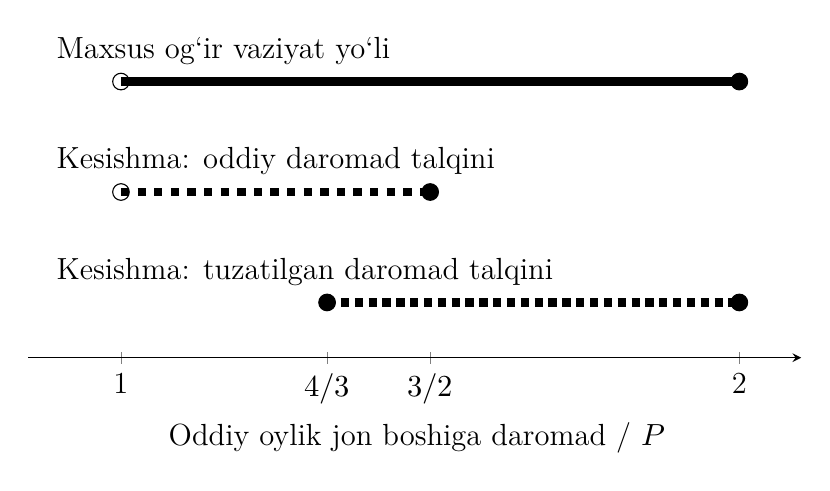
\begin{tikzpicture}
\begin{axis}[width=.94\linewidth,height=6cm,xmin=.85,xmax=2.1,ymin=.5,ymax=3.65,xtick={1,1.333333333,1.5,2},xticklabels={1,$4/3$,$3/2$,2},ytick=\empty,axis y line=none,axis x line=bottom,xlabel={Oddiy oylik jon boshiga daromad / $P$}]
\addplot[black,line width=3pt] coordinates {(1,3)(2,3)};
\addplot[black,line width=3pt,dashed] coordinates {(1,2)(1.5,2)};
\addplot[black,line width=3pt,dotted] coordinates {(1.333333333,1)(2,1)};
\addplot[only marks,mark=*,mark size=3pt] coordinates {(2,3)(1.5,2)(1.333333333,1)(2,1)};
\addplot[only marks,mark=o,mark size=3pt,mark options={fill=white}] coordinates {(1,3)(1,2)};
\node[anchor=west] at (axis cs:.88,3.28) {Maxsus og‘ir vaziyat yo‘li};
\node[anchor=west] at (axis cs:.88,2.28) {Kesishma: oddiy daromad talqini};
\node[anchor=west] at (axis cs:.88,1.28) {Kesishma: tuzatilgan daromad talqini};
\end{axis}\end{tikzpicture}
\end{center}
\textbf{1-rasm.} Daromad P ga nisbatan olingan. To‘ldirilgan nuqta chegara kirishini, ochiq nuqta kirmasligini ko‘rsatadi. Maxsus yo‘l tegishli holat, tavsiya, kvota va boshqa qonuniy shartlarni ham talab qiladi. Kesishmalar talqin farqi, kuzatilgan rad etishlar emas.

\subsection{Yer formulasining kirish sohasi auditi}
$U\leq1,000$ bo‘lsa $L=4U/5-B$; L faqat $B>4U/5$ da manfiy. $U>1,000$ bo‘lsa $L=U-B-200$; faqat $B>U-200$ da manfiy. Bu tengsizliklar sanashni mustaqil tekshiradi. $0\leq B\leq U$ da L ning pastki chegarasi $-\min(U/5,200)$. Fizik maydon manfiy bo‘la olmaydi, ammo amaliy kadastr cheklovlari tuzilgan kirishlarni maqbul yozuvlardan chiqarishi mumkin.

\begingroup\fontsize{11bp}{13.2bp}\selectfont
\begin{longtable}{p{\dimexpr\linewidth/5-2\tabcolsep\relax} p{\dimexpr\linewidth/5-2\tabcolsep\relax} p{\dimexpr\linewidth/5-2\tabcolsep\relax} p{\dimexpr\linewidth/5-2\tabcolsep\relax} p{\dimexpr\linewidth/5-2\tabcolsep\relax}}
\toprule
U maydon (m²) & Butun qiymatli misollar & Manfiy misollar & Eng kam L (m²) & Eng ko‘p chegara farqi (so‘m/oy) \\
\midrule
\endhead
100 & 101 & 20 & -20 & 9,520 \\
1,000 & 1,001 & 200 & -200 & 95,200 \\
1,001 & 1,002 & 200 & -200 & 95,200 \\
2,000 & 2,001 & 200 & -200 & 95,200 \\
Tuzilgan to‘r jami & 4,105 & 620 & — & — \\
\bottomrule
\end{longtable}
\endgroup
\textbf{1-jadval.} Sentabr uchun M = 1,360,000 va faraziy diagnostik k = 1 bilan hisoblangan. Sonlar tuzilgan to‘r xususiyatlari. Oxirgi ustun hisoblangan oylik oila daromadining o‘zgarishi; to‘lov kamayishi yoki fiskal baho emas.

U = 100, B = 90 da L = −10 m², literal oylik daromad −4,760 so‘m. Taklif etilgan nol chegara nol beradi. Belgilangan sohada chegara sentabr M bilan oylik normativ daromadni eng ko‘p 95,200k ga oshirishi mumkin; N ga bo‘lish jon boshiga ulushni beradi. Manfiy ulushni tuzatish daromadni oshirishi mumkin; uni yordamni avtomatik ko‘paytiradi deb bo‘lmaydi. Haqiqiy toifa va to‘lov ta’siri qonuniy oldin/keyin takrorlash va tegishli yordam qoidalarini talab qiladi.

Nol pastki chegara matematik asoslangan taklif, lekin geometriya ta’rifini almashtirmaydi. Kadastr B bino izi ekanini, qaysi obyektlarni qamrashini, chegiriladigan maydonlar ustma-ust tushishini va U, B bir uchastka va sanaga tegishliligini aniqlashi kerak. Agar 20 foiz muayyan foydalanish maydonini anglatsa, ustma-ust tushmaydigan fizik konstruksiya afzal bo‘lishi mumkin. Ma’noni ishlab chiquvchi belgilaydi; audit kadastr faktini o‘ylab topmaydi.

\begin{center}
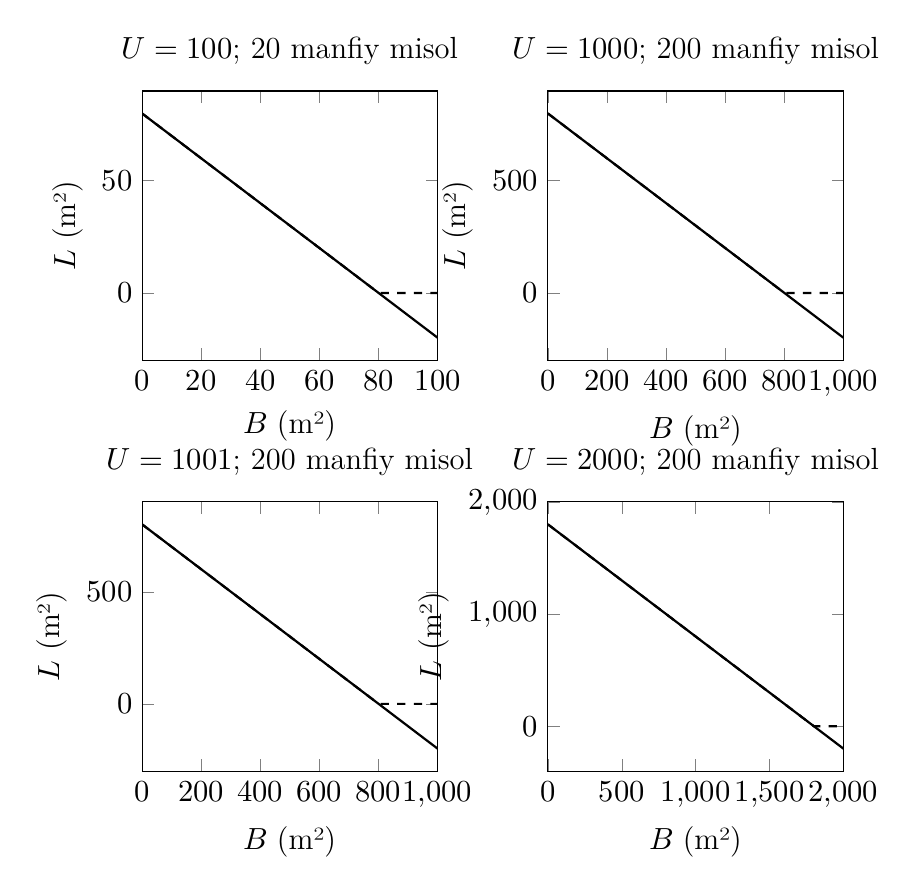
\begin{tikzpicture}
\begin{groupplot}[group style={group size=2 by 2,horizontal sep=1.4cm,vertical sep=1.8cm},width=.44\linewidth,height=5cm,xlabel={$B$ (m²)},ylabel={$L$ (m²)},scaled ticks=false]
\nextgroupplot[title={$U=100$; 20 manfiy misol},xmin=0,xmax=100]
\addplot[black,thick] coordinates {(0,80)(100,-20)};
\addplot[black,dashed,thick] coordinates {(0,80)(80,0)(100,0)};
\nextgroupplot[title={$U=1000$; 200 manfiy misol},xmin=0,xmax=1000]
\addplot[black,thick] coordinates {(0,800)(1000,-200)};
\addplot[black,dashed,thick] coordinates {(0,800)(800,0)(1000,0)};
\nextgroupplot[title={$U=1001$; 200 manfiy misol},xmin=0,xmax=1001]
\addplot[black,thick] coordinates {(0,801)(1001,-200)};
\addplot[black,dashed,thick] coordinates {(0,801)(801,0)(1001,0)};
\nextgroupplot[title={$U=2000$; 200 manfiy misol},xmin=0,xmax=2000]
\addplot[black,thick] coordinates {(0,1800)(2000,-200)};
\addplot[black,dashed,thick] coordinates {(0,1800)(1800,0)(2000,0)};
\end{groupplot}\end{tikzpicture}
\end{center}
\textbf{2-rasm.} Har panel oldindan belgilangan U va noldan U gacha barcha butun B ni ishlatadi. Vertikal o‘q m² dagi hosila maydon. Manfiy qism literal formulaga tegishli; uzilgan chiziq taklif etilgan nol chegarani alohida ko‘rsatadi. Grafik ma’muriy kuzatuv qo‘shmaydi.

\subsection{Pul o‘tkazmalari birliklari va shartli uzilishlar}
q = 2M tenglik pastki chegaradan kam shartni qanoatlantirmaydi. Oylik talqinda ro‘yxatdagi guruh chegaradan sal pastdagi 3M dan tenglikdagi 2M ga o‘tadi: oyiga M = 1,360,000 so‘m pasayish. Boshqa guruh 2M dan 2M ga o‘tib, uzluksiz. Uch oylik yig‘indi talqinida haqiqiy daromad tenglikda oyiga 2M/3; pasayish boshqacha. O‘n olti tuzilgan misol ikki talqin, ikki guruh va yo‘q qiymat shoxini saqlaydi.

\begingroup\fontsize{11bp}{13.2bp}\selectfont
\begin{longtable}{p{\dimexpr\linewidth/4-2\tabcolsep\relax} p{\dimexpr\linewidth/4-2\tabcolsep\relax} p{\dimexpr\linewidth/4-2\tabcolsep\relax} p{\dimexpr\linewidth/4-2\tabcolsep\relax}}
\toprule
Shartli davr & Mamlakat guruhi & Oylik ulush pasayishi (so‘m) & 4 a’zoda jon boshiga pasayish (so‘m) \\
\midrule
\endhead
Oylik & Ro‘yxatdagi mamlakatlar & 1,360,000 & 340,000 \\
Oylik & Boshqa mamlakatlar & 0 & 0 \\
Uch oylik yig‘indi & Ro‘yxatdagi mamlakatlar & 9,520,000/3 & 2,380,000/3 \\
Uch oylik yig‘indi & Boshqa mamlakatlar & 5,440,000/3 & 1,360,000/3 \\
\bottomrule
\end{longtable}
\endgroup
\textbf{2-jadval.} So‘mdagi aniq shartli arifmetika. Qiyoslash davri hal qilinmagan; hech bir qator amaldagi ijro topilmasi emas. Son daromad ulushi o‘zgarishi, yordam summasi emas.

Ro‘yxatdagi mamlakatlar oylik qoidasi normativdan haqiqiyga o‘tishda monoton emas: kattaroq bildirilgan qiymat kichikroq hisoblangan ulush berishi mumkin. Bu albatta matn xatosi degani emas; zaxira baho va kuzatilgan qiymat ataylab farqlanishi mumkin. Ammo ilmiy-huquqiy izoh, takrorlanadigan manba ishlovi va toifa o‘zgarishini baholash talab etadi. Dasturchi qoida o‘rniga yashirin $\max(haqiqiy,normativ)$ qo‘ya olmaydi; bu uning mazmunini o‘zgartiradi.

Yo‘q qiymat va qayd etilgan nol bir normativ summa bersa ham alohida holat bo‘lishi kerak: sababi, dalili va tuzatishi farqli. Manba davri, yuboruvchilar bo‘yicha yig‘ish, kurs sanasi va zaxira qoida sababi saqlanadi. Grafikni silliqlash uchun davr yoki pastki chegara tanlash dalilsiz siyosiy tanlov bo‘ladi.

\begin{center}
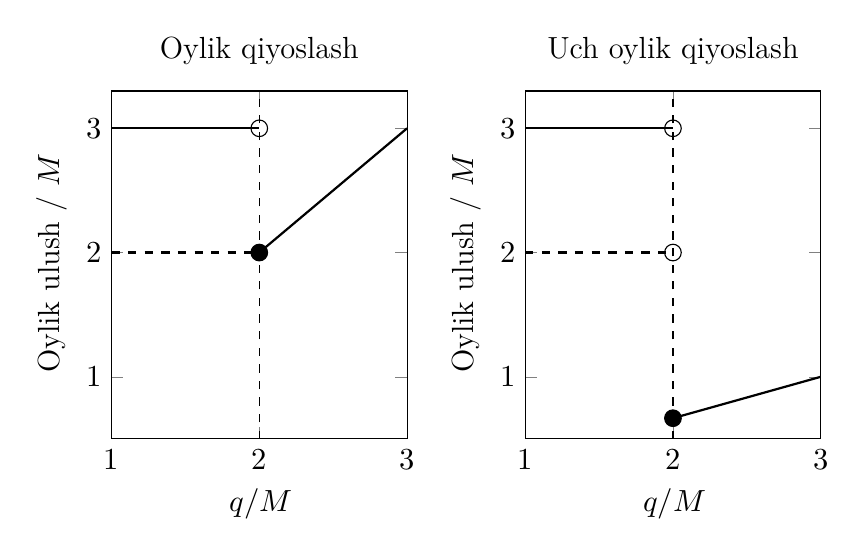
\begin{tikzpicture}
\begin{groupplot}[group style={group size=2 by 1,horizontal sep=1.5cm},width=.44\linewidth,height=6cm,xmin=1,xmax=3,ymin=.5,ymax=3.3,xtick={1,2,3},ytick={1,2,3},xlabel={$q/M$},ylabel={Oylik ulush / $M$}]
\nextgroupplot[title={Oylik qiyoslash}]
\addplot[black,thick] coordinates {(1,3)(2,3)};
\addplot[black,dashed,thick] coordinates {(1,2)(2,2)};
\addplot[black,dashed] coordinates {(2,.5)(2,3.3)};
\addplot[black,thick] coordinates {(2,2)(3,3)};
\addplot[only marks,mark=*,mark size=3pt] coordinates {(2,2)};
\addplot[only marks,mark=o,mark size=3pt,mark options={fill=white}] coordinates {(2,3)};
\nextgroupplot[title={Uch oylik qiyoslash}]
\addplot[black,thick] coordinates {(1,3)(2,3)};
\addplot[black,dashed,thick] coordinates {(1,2)(2,2)};
\addplot[black,dashed] coordinates {(2,.5)(2,3.3)};
\addplot[black,thick] coordinates {(2,.666666667)(3,1)};
\addplot[only marks,mark=*,mark size=3pt] coordinates {(2,.666666667)};
\addplot[only marks,mark=o,mark size=3pt,mark options={fill=white}] coordinates {(2,3)(2,2)};
\end{groupplot}\end{tikzpicture}
\end{center}
\textbf{3-rasm.} Gorizontal q/M, vertikal oylik ulush/M. Uzluksiz gorizontal chiziq ro‘yxatdagi, uzilgan gorizontal chiziq boshqa mamlakatlar; haqiqiy qiymat yo‘li ikkalasida bir xil. Ikki panel ikki davr talqinini saqlaydi. Vertikal uzilgan chiziq qiyoslash chegarasi. Yo‘q qiymat JSONda qayd etilgan, sonli nuqta sifatida chizilmagan.

\subsection{Koeffitsiyentlar, soliq minimumi va kasrli chorva}
23-band to‘rt hudud va ikki jins bo‘yicha sakkiz oylik o‘zini o‘zi band qilish koeffitsiyentini beradi. Sentabr M bilan erkak–ayol farqi har sinfda 0.4M = 544,000 so‘m. Tuzilgan to‘rt kishilik oilada bitta shunday a’zo jon boshiga 136,000 farq kiritadi. Bu normativ daromad sezgirligi; haqiqiy ish haqi, kamsitish, teng bo‘lmagan huquq yoki xato darajasi o‘lchovi emas. Koeffitsiyentni empirik asoslash va huquqiy tenglikni tekshirish alohida dalil talab qiladi.

\begingroup\fontsize{11bp}{13.2bp}\selectfont
\begin{longtable}{p{\dimexpr\linewidth/5-2\tabcolsep\relax} p{\dimexpr\linewidth/5-2\tabcolsep\relax} p{\dimexpr\linewidth/5-2\tabcolsep\relax} p{\dimexpr\linewidth/5-2\tabcolsep\relax} p{\dimexpr\linewidth/5-2\tabcolsep\relax}}
\toprule
Hudud sinfi & Erkak bazasi & Ayol bazasi & Norasmiy erkak & Norasmiy ayol \\
\midrule
\endhead
Toshkent & 3,672,000 & 3,128,000 & 3,855,600 & 3,284,400 \\
Nukus / viloyat markazlari & 3,264,000 & 2,720,000 & 3,427,200 & 2,856,000 \\
Boshqa shaharlar & 2,856,000 & 2,312,000 & 2,998,800 & 2,427,600 \\
Boshqa birliklar & 2,448,000 & 1,904,000 & 2,570,400 & 1,999,200 \\
\bottomrule
\end{longtable}
\endgroup
\textbf{3-jadval.} M = 1,360,000 bilan hisoblangan ulushlar. Norasmiy daromad tegishli baza 1.05 ga ko‘paytiriladi, faqat 25-band shartlari mavjud bo‘lsa. Haqiqiy oila tarkibi haqida xulosa qilinmaydi.

24-band soliq ifodasi $T=3B_0/2.5=6B_0/5$ da bazaga teng. Pastda natija $B_0$, yuqorida uch oylik soliq yig‘indisiga nisbatan 5/6 qiyalik bilan oshadi. Yigirma to‘rt oldindan belgilangan sinov bo‘lakli ifodaga mos. Minimum uzluksiz va monoton; ro‘yxatdagi mamlakat pul o‘tkazmasi almashuvi kabi emas. Shuning uchun bitta umumiy «chegara sezgirligi» soni barcha qoidani tavsiflamaydi.

O‘n to‘rt echki uchun daromad nol: $14\times0.07=0.98$ shartli bosh. O‘n beshta — 1.05 bosh, hisoblanadigan 0.05 bosh va oyiga 34,000 so‘m. Yigirmata — 272,000; yuzta — 4,080,000. Istisnoni qo‘llashdan oldin shartli boshni pastga yaxlitlash bu natijani o‘zgartiradi va bu yerda kodlangan qoida emas. Rasmiy yaxlitlash spetsifikatsiyasi kasrli boshlarni hal qilishi kerak. Boshqa turlar va aralash podalar amalga oshirilmagan.

\subsection{Son tanlash bilan hal qilinmagan spetsifikatsiya masalalari}
Ikki hujjat masalasi afzal sonni tanlamasdan aniqlashtiriladi. Birinchisi: tayanch oylar chegarasi va kechikishi 18-band va 30-band misoliga mos bo‘lishi kerak. Ikkinchisi: 20-band umumiy subsidiya chiqarishlari va 29-band qayta tiklanadigan elektr savdosi QP subsidiyasini kiritishi uchun ustuvorlik yozuvi kerak. Maxsus kiritish umumiy chiqarishdan qonuniy ustun bo‘lishi mumkin. Ish QP noqonuniy yoki tizim uni ikki marta hisoblaydi deb da’vo qilmaydi; ikkala savol ham o‘zboshimcha dastur faraziga aylantirilmagan.

\section{Taklif etilgan normalar va ularning huquqiy asoslari}
\subsection{Hujjat tuzilishi va yuridik kuch}
1-materialdagi normativ loyiha yettita asosiy band va yigirma sakkiz bandli ilovadan iborat. Asosiy talab — huquqiy oqibatli hisoblash tasdiqlangan uslubiyotga mosligini tekshirish, asosini saqlash va yangi rad etish asosi yaratmasdan hal qilinmagan holatni ko‘rsatish. Tahrir texnik qabul qilish vakolati, aniq qabul mezonlari, amal qilish sanalari va qonuniy saqlash jadvalini belgilaydi. U amaldagi tizimni to‘ldiradi. Yakuniy hujjat turi, mablag‘ va bog‘liq o‘zgartirishlarni vakolatli ishlab chiquvchi aniqlaydi.

Tenglik uchun taklif Prezident va Hukumat normalarini birgalikda o‘zgartirishni nazarda tutadi. Yerning nol chegarasi 35-son qaror formulasini o‘zgartirishdir. Qolganlari tekshirish va kuzatuv talablaridir. Ularning qabul qilish shartlari turlicha; barchasini oddiy dastur sozlamasi deb bo‘lmaydi. O‘RQ-682 18-moddasi yuridik kuch nisbatini belgilaydi. \cite{ref7}.

\begingroup
\fontsize{11bp}{13.2bp}\selectfont
\begin{longtable}{p{\dimexpr\linewidth/4-2\tabcolsep\relax} p{\dimexpr\linewidth/4-2\tabcolsep\relax} p{\dimexpr\linewidth/4-2\tabcolsep\relax} p{\dimexpr\linewidth/4-2\tabcolsep\relax}}
\toprule
Audit topilmasi yoki talab & Taklif ilovasi bandlari & Muvofiqlashtiriladigan qoidalar & Taklif mohiyati \\
\midrule
\endhead
Tenglik va maxsus yo‘l ustuvorligi & 5, 12, 16 & PF-258 3-band va 1-ilova izohlari; 35-son qaror 32–35, 39, 42-bandlar & Ixtiyoriy toifa tuzatishi; qonuniy yo‘lning zarur spetsifikatsiyasi \\
Manfiy yer maydoni & 4, 12 & 35-son qaror 27-band; kadastr maydonlari & Ixtiyoriy formula tuzatishi; zarur geometriya/manba ta’rifi \\
Tayanch davr va o‘tkazma birliklari & 4, 8 & 35-son qaror 18–19, 21, 26, 29–30-bandlar & Aniq birlik, davr va yig‘ish qoidalari \\
Manba uzilishi va vaqtinchalik algoritm & 8–11, 18 & 35-son qaror 48-band; almashinuv ilovalari & Kuzatiladigan vaqtinchalik versiya va keyingi tekshiruv \\
Mustaqil hisob va hal qilinmagan holat & 12–17 & Reyestr, qayta baholash, to‘lov qoidalari & Oldindan belgilangan tekshiruv, alohida maxrajlar \\
Asoslar, tuzatish va ko‘rib chiqish & 18–20 & SMS/qayta baholash va shikoyat tartiblari & Qonuniy jarayonda hisoblash asosini olish \\
Himoyalangan tadqiqot va umumlashtirilgan hisobot & 21–24 & Shaxsga doir ma’lumotlar qonuni; nazorat vakolati & Qonuniy ichki bajarish va oshkor etishni tekshirish \\
Qabul qilish, o‘tish va saqlash & 25–28 & Tasdiqlangan uslubiyot, amal sanalari, to‘lov va saqlash qoidalari & Siyosat vakolatini bermasdan yozma texnik qabul \\
\bottomrule
\end{longtable}
\endgroup
\textbf{4-jadval.} Ilmiy natijadan taklif etilgan normaga bog‘lanish. Bandlar amaldagi qonunchilik emas, muallif ilovasi raqamlari. Muvofiqlashtirish ishlab chiquvchi vazifasi; jadval barcha bog‘liq dastur normalarining to‘liq ro‘yxati emas.

\subsection{Uslubiyot pasporti}
Har huquqiy oqibatli o‘zgaruvchi pasportida maqsad, vakolatli manba, oila/shaxs bog‘lanishi, birlik, tayanch davr, maqbul oraliq, o‘tkazish, yo‘q/zid/eskirgan qiymatga ishlov va amal sanali parametr ko‘rsatilishi kerak. O‘lchangan qiymat normativ hisoblangan miqdordan ajratiladi. «Oxirgi yangilanish»ning o‘zi yetmaydi: eski yozuv kerakli davrni, yangi kelgan yozuv noto‘g‘ri davrni tasvirlashi mumkin.

Toifa spetsifikatsiyasi qaror jadvali yoki teng formal qoidalar bilan ifodalanadi. Har qator qo‘llanish, ustuvorlik, shart, natija va huquqiy asosni ko‘rsatadi. Maxsus yo‘l tegishli holatlar, tavsiya, kvota va qayta baholashni saqlashi kerak; daromad formulasining o‘zi kirish huquqini bermaydi. Dastlabki e’tirof, reyestr toifasi, dastur huquqi va summa alohida yoziladi. Hal qilinmagan holat qonuniy hal etishni talab qiladigan texnik maqom; o‘ylab topilgan to‘rtinchi yordam toifasi emas.

Model va dastur versiyasi, manba nusxalari, davrlar, qo‘llangan istisnolar va hisoblash bosqichlari qayd etiladi. Qonun bilan himoyalangan ma’lumotdan tashqari tavsif ochiq bo‘lishi kerak. Cheklangan material vakolatli tekshiruvchi va ko‘rib chiquvchilarga ochiq qoladi. Bu takrorlash va maxfiylikni muvozanatlashtiradi; tashqi muallifga mikroma’lumot olish huquqi bermaydi.

\subsection{Qabul qilinishi taklif etilgan talablar}
Agentlik Vazirlik bilan tasdiqlanadigan spetsifikatsiyani tayyorlashi, birinchi qo‘llash va muhim o‘zgarishdan oldin tekshirishi, bayonnomani saqlashi taklif etiladi. Muhim o‘zgarish hisoblash yoki toifaga ta’sir qilishi mumkin bo‘lgan, jumladan manba bog‘lanishi yoki davrga o‘tkazishdagi o‘zgarishdir. Mazmuni bir xil maydon nomini almashtirish muhim bo‘lmasligi mumkin. Ilova 25-bandi uslubiyot, axborot tizimi va yuridik xizmat xulosalari asosida texnik qabulni Agentlik rahbari yoki qonuniy vakolatlangan o‘rinbosariga yuklaydi. Bu taklif, amaldagi tayinlash dalili yoki ball mezonlarini belgilash vakolati emas.

26-band qabulni tekshiriladigan qiladi. Oldindan belgilangan har chegara va istisno misolining qonuniy kutilgan natijasi bo‘lishi kerak; bir tasdiqlangan versiya va aynan bir kirish uchun tasdiqlangan yaxlitlashdan keyin ball yoki toifa tafovuti bo‘lmasligi; sifat, izoh olish va e’tirozni yo‘naltirish vazifalari ishlashi kerak. Xato tuzatilib, tegishli sinovlar qaytariladi. Bu muvofiqlik mezoni, aholi bo‘yicha aniqlik nishoni emas. Farovonlik mezoni va tanlanma yo‘q paytda 95 foizlik ixtiyoriy aniqlik talabini qonunga kiritish asoslanmagan. Talab qonuniy ariza ishlovini yoki belgilangan joriy etish sanasini o‘zgartirmaydi.

Tenglik, istisno, yetishmaydigan ma’lumot va fizik jihatdan yaroqsiz hosilalar sinovdan o‘tkaziladi. Hal qilinmagan holatni muvaffaqiyatli maxrajda yashirish yoki sintetik sinovni farovonlik tekshiruvi deyish taqiqlanadi. Dastur tasdiqlangan qoidaga zid bo‘lsa, ta’sirlangan hisoblashlar ko‘rib chiqiladi. Individual tuzatish, to‘lov davomiyligi va shikoyat muddati amaldagi qonunga bo‘ysunadi; modul avtomatik to‘xtatish vakolati bermaydi.

\begin{sloppypar}
35-son qaror 48-bandi axborot almashinuvi uzilganda vaqtinchalik algoritmni o‘zgartirishga ruxsat beradi. Taklif bu vakolatni saqlab, huquqiy asos, doira, boshlanish vaqti, vaqtinchalik qoida va tiklash shartini yozishni talab qiladi. O‘sha versiya hisoblashlari keyingi qonuniy tekshirish uchun ajratiladi. Parallel favqulodda organ yaratilmaydi. 49-banddagi nazorat vazifalari ham tayanchdir.
\end{sloppypar}

Izoh qaror nima uchun chiqqanini, normativ hisoblash va istisno mantiqini ochadi. SMSning o‘zi hisoblashni takrorlamaydi. Ma’muriy tartib-taomillar qonuni 53–54-moddalari individual ma’muriy hujjat mazmuni va faktik-huquqiy asoslarini tartibga soladi; aynan tegishli qaror uchun qo‘llanish va maxsus tartib tekshirilishi kerak. Taklif 19-bandi qaror bilan birga shaxsiy kabinetda asosni taqdim etish, undan foydalanmaydigan shaxsga «Inson» markazi orqali kirishni beradi. Bu yangi taklif etilgan majburiyat; amaldagi interfeysda allaqachon mavjudligi haqidagi da’vo emas. \cite{ref10}.

\subsection{Qabul dalili, mustaqil javob va sinov qamrovi}
Muvaffaqiyatli sinov uchun faqat ikkita mos natija emas, mustaqil asoslangan kutilgan javob kerak. Barr va hammualliflar sinovning to‘g‘ri javobini aniqlash muammosini tushuntirib, spetsifikatsiyadan chiqarilgan javobni boshqa dastur bilan qiyoslashdan ajratadi. NIST IR 8397 talabdan chiqarilgan sinov, kod tuzilishidan chiqarilgan sinov va oldingi nuqsonlar uchun saqlangan regressiya misolini farqlaydi. Bu manbalar tekshirishning muhandislik tuzilishini qo‘llab-quvvatlaydi; O‘zbekistonda yordamga huquqning majburiy standarti emas. Ular loyiha misollari Agentlik tizimini to‘liq qamraganini isbotlamaydi. \cite{ref21}; \cite{ref22}.

Taklif bo‘yicha uslubiyot bo‘linmasi va yuridik xizmat kutilgan natijaning huquqiy chiqarilishini belgilashi; sinalayotgan dasturni amalga oshirish uchun mas’ul shaxsdan boshqa tekshiruvchi uni tekshirishi kerak. Qaydda manba normasi va tahriri, yo‘lning dastlabki shartlari, kirish birliklari va davrlari, oraliq hissalar, yaxlitlash bosqichi va yakuniy natija ko‘rsatiladi. Masalan, $D=P$ da $\leq P$ qo‘llaydigan dastur javobini ko‘chirish e’lon qilingan qat’iy $<P$ toifa shartiga nomuvofiqlikni yashiradi. Aksincha, og‘ir vaziyat yo‘liga umumiy pastki chegara kiritish saqlangan $0.75D=P$ qarshi misolini chiqarib tashlaydi. Kod qoidaga mosligi va qoidani o‘zgartirish zarurati ikki alohida savoldir. Hal etilmagan talqin qonuniy yechim uchun yuboriladi; dasturlar mosligi yoki ko‘pchilik ovozi uni hal qilmaydi.

Ilovaning 12 va 26-bandlari endi tanlangan sinovlar to‘liqlikni o‘zi belgilashiga yo‘l qo‘ymay, qoida va misol bog‘lanishi ro‘yxatini talab qiladi. Har bir qo‘llanadigan chegara, istisno, ustuvorlik yo‘li va amalga oshishi mumkin bo‘lgan birikmaning kutilgan natijasi bo‘ladi; qo‘llanmaydigan yo‘lni chiqarish asoslanadi. Bajarishdan oldin misol identifikatorlari va kirish qiymatlari qat’iy belgilanadi. So‘ng bajarilgan misollar ro‘yxat bilan solishtiriladi, yetishmaydigan yoki takrorlangan identifikatorlar hisobga olinadi. To‘liq bo‘lmagan ro‘yxatdagi ijobiy natija e’lon qilingan doira bajarilganini anglatmaydi. Kod qamrovi qo‘shimcha dalil beradi, ammo bajarilgan satrlar foizi tushirilgan huquqiy norma qamrovini isbotlamaydi.

\begingroup\fontsize{11bp}{13.2bp}\selectfont
\begin{longtable}{p{\dimexpr\linewidth/3-2\tabcolsep\relax} p{\dimexpr\linewidth/3-2\tabcolsep\relax} p{\dimexpr\linewidth/3-2\tabcolsep\relax}}
\toprule
Qoidalar guruhi & Bajarilgan tekshiruv va doira & Agentlikdan talab etiladigan qo‘shimcha qabul dalili\\
\midrule\endhead
Asosiy daromad shartlari & 10 sun’iy qator; bitta avvalgi toifa nazorati; mehnatga layoqatli arizachi shartlari & Boshqa rad asoslari, mehnatga layoqat yo‘llari, a’zolik sanasi va e’tirof/toifa ustuvorligi.\\
Og‘ir vaziyat yo‘li & 12 chegara qatori va alohida belgilangan bitta keyingi qarshi misol & Tegishli vaziyat, qonuniy tavsiya, kvota, qayta baholash va asosiy/avvalgi toifa yo‘llari bilan birikish.\\
Yer & To‘rtta umumiy maydon uchun 4\,105 butun sonli holat; mahalliy koeffitsiyent 1 & Bir uchastkaning vakolatli geometriyasi, kasrli maydonlar, sanali mahalliy koeffitsiyent, manba cheklovi va yaxlitlash.\\
Soliq minimumi & Sakkiz hudud/jins katagida 24 kesishish qatori & Soliq yig‘indisining ma’nosi va to‘liqligi, davrlar, o‘zgaruvchi parametrlar va manba istisnolari.\\
Pul o‘tkazmalari & Ikki shartli davr va ikki mamlakat guruhi bo‘yicha 16 qator & Bitta qonuniy aniqlangan qiyoslash davri, jo‘natuvchilarni jamlash, takrorlar, valuta aylantirish va manba maqomi.\\
Chorva & Faqat echkilardan iborat oltita holat, aniq kasrli aylantirish & Boshqa tur, aralash chorva, istisno, davr va tasdiqlangan yaxlitlash; bu yerda amalga oshirilmagan.\\
Additiv namuna & Yetti sun’iy holat; belgilab berilgan toifalar bilan to‘rtta qiyoslanadigan holat & Rasmiy formula, kirish sohasi/bog‘liqlik, istisno va qonuniy kirishlar. Namuna noma’lum nochiziqli modelni tasdiqlamaydi.\\
\bottomrule
\end{longtable}
\endgroup
\textbf{5-jadval.} Bajarilgan doira va hal etilmagan amaliy shartlar. Sonlar oilalar emas, tuzilgan misollarni bildiradi. Bu qabul dalillari ro‘yxati, qo‘shimcha ish bajarilgani da’vosi emas.

Jami ball va toifa mos bo‘lsa ham oraliq tarkibiy qiymatlar tekshiriladi. Tushirib qoldirilgan hissa va xato qo‘shimcha hissa jamida bir-birini qoplashi mumkin. Nazorat kiritish/chiqarish sabablari, manba davrlari, aylantirish va yaxlitlashni ham qiyoslaydi. Qayd tasdiqlangan huquqiy uslubiyotni dasturiy chiqarilish, moslashtirish/sozlama va sanali parametrlardan; huquqiy amal sanasini joriy etish sanasidan ajratadi. O‘zgarmagan huquqiy qoidani bajaruvchi tuzatilgan dastur o‘sha qoida identifikatorini saqlab, alohida dasturiy qayd oladi. Qaror kirishlari yoki qonuniy saqlangan nusxa tarixiy takrorlashni ta’minlaydi; o‘zgarib turadigan jonli bazaga havolaning o‘zi yetarli emas.

Yangilangan mustaqil tekshiruvchi qat’iy misol identifikatorlari va takrorlanish sonini tekshiradi hamda o‘nta daromad sharti qatorini mustaqil tekshiradi. Oltita qo‘shimcha regressiya sinovi bo‘sh ro‘yxatni, qator sonini o‘zgartirmasdan misol o‘rniga takror qo‘yilishini, o‘zgartirilgan tenglik shartini va boshqa qat’iy misol deb ko‘rsatilgan kirishni hamda misol identifikatoriga majburan aylantirilgan kasrli yoki mantiqiy kirishni rad etadi hamda o‘zgarmagan hisobotni qabul qiladi. To‘liq to‘plam endi 37 sinovdan iborat. Bu tekshiruvchining isbotlangan nuqsonini tuzatadi: ilgari og‘ir vaziyat, soliq, o‘tkazma va echki ro‘yxatlari bo‘sh bo‘lsa ham muvaffaqiyat yorlig‘iga yetish mumkin edi. O‘zgarmagan sonli natijalar kuchaytirilgan tekshiruvdan o‘tdi. Bu bilan amaliy dastur yoki oilalar tanlanmasi tasdiqlanmaydi.

\subsection{Shikoyat vakolati: amaldagi kengash doirasi}
35-son qaror 4-ilova 26-bandi apellatsiya kengashini reyestr arizasida mahalla yettiligi tuzgan savolnoma, xulosa va dalolatnomalar bilan chegaralaydi. 31-band shu doiradan tashqari shikoyatni rad etishga imkon beradi. Sof hisoblash nizosini shunchaki kengash shikoyati deb uning vakolatiga kiritib bo‘lmaydi. Bu aniq yo‘lning doirasi; boshqa ma’muriy yoki sud yo‘li yo‘qligini ko‘rsatmaydi. 33-band kengash uchun o‘n besh kunlik ko‘rib chiqishni belgilaydi. \cite{ref2}.

Shaxsga doir ma’lumotlar qonuni alohida yo‘l beradi. 24-modda o‘z istisnolarida faqat avtomatik huquqiy oqibatli qarorga ruxsat berib, mulkdor/operatorga tartib va oqibatni tushuntirish, e’tiroz imkonini berish va natijani o‘n kun ichida yozma xabar qilishni yuklaydi. Bu manba yozuvini tuzatish yoki mahalla hujjatini nizolashdan farq qiladi. 11-modda subyekt talabi bo‘yicha tuzatish/to‘ldirishni uch kun ichida, aniqlangan noto‘g‘ri ma’lumotni darhol tuzatishni talab qiladi; bu muddatni avtomatik qaror e’tirozining o‘n kuniga almashtirib bo‘lmaydi. Taklif 20-bandi avtomatik qaror e’tirozini mulkdor/operatorga, manba tuzatishini vakolatli manbaga, kengash shikoyatini uning qonuniy doirasiga yo‘naltiradi. Boshqa qonuniy yo‘llar saqlanadi, qo‘shimcha majburiy sudgacha bosqich yaratilmaydi. Dastur normasi kengash vakolatini o‘zi kengaytirayotgandek ko‘rsatilmaydi. \cite{ref9}.

Ishlab chiquvchi qabul shakllari va yuborish tartibini farqli yo‘llarga moslashtiradi. Ochiq tushuntirish har yo‘lning vakolatli oluvchisi, predmeti va muddatini ko‘rsatadi. Bir nechta savol bo‘lsa dastlabki qabul yozuvi saqlanib, alohida yo‘naltiriladi; yuborish qonuniy muddatni yangidan boshlamasligi kerak. Bu mavjud kafolatlarni ishlatish uchun taklif etilgan jarayon; muallif yaratgan umumiy shikoyat huquqi emas.

\subsection{O‘tish, tuzatish va qonuniy saqlash}
Uch operatsiya ajratiladi: yangi siyosat qoidani kelajak uchun o‘zgartiradi; dastur tuzatishi oldingi qarorga qo‘llangan qoidaning ijrosini tuzatadi; manba tuzatishi muayyan davr dalilini o‘zgartiradi. 27-band keyingi parametr yoki yangi mezonni tarixiy hisobga avtomatik qo‘llashni taqiqlaydi. Qayta hisoblashning o‘zi qaytarib undirish asosi emas. Undirish yoki individual qarorning salbiy o‘zgarishi tegishli moddiy va protsessual asosni talab qiladi. Ma’muriy tartib-taomillar qonuni 59–61-moddalaridagi talablarni hisobga olganda, texnik ilovada shartsiz undirish yoki undirishdan shartsiz daxlsizlikni va’da qilish huquqiy jihatdan asoslangan xulosa bo‘lmaydi. \cite{ref10}.

Eski hisobni saqlash ko‘rib chiqish uchun kerak, ammo barcha shaxsiy yozuvni cheksiz saqlashga asos emas. 28-band har toifa uchun qonuniy asos, muddat, vakolatli kirish, tuzatish tarixi va tegishli qonuniy yo‘q qilish yoki egasizlantirishni talab qiladi. Shaxsga doir ma’lumotlar qonuni 17-moddasi arxiv majburiyatlari bilan birga qo‘llanadi; majburiy yo‘q qilishni egasizlantirish bilan almashtirib bo‘lmaydi. Aniq jadval Agentlik yozuv inventariga bog‘liq; o‘ylab topilgan yil muddati berilmaydi. Ochiq natijalar jadvallararo oshkor etish tekshiruvini talab qiladi: alohida zararsiz agregatlar bog‘langanda kichik oila guruhini aniqlashi mumkin. \cite{ref9}.

\subsection{22-modda bo‘yicha loyihani tayyorlashda ishtirok}
20-modda masalani mavjud qonuniy mexanizm va ma’muriy vakolat bilan hal etish mumkin bo‘lganda unda ko‘rsatilgan loyihalarni tashabbus qilishni cheklaydi. Taklif PF-193-son Farmonning 14-bandi bilan allaqachon topshirilgan loyihaga hissa sifatida kiritiladi; topshiriq aynan ushbu bandlarni kiritish majburiyatini bermaydi. Har vazifa mavjud vakolat yoki vakolatli hujjatni talab etuvchi yangi majburiyat bilan bog‘lanishi kerak. Ichki tekshiruv yo‘riqnomasi mavjud vakolatdan foydalanishi mumkin; yuqori yuridik kuchdagi mezonni dastur sozlamasi yoki quyi hujjat o‘zgartira olmaydi. Tekshiruv moduli va ixtiyoriy siyosiy o‘zgartirishlar alohida hal qilinadi. \cite{ref1}; \cite{ref7}.

23-modda ishlab chiquvchidan tegishli tadqiqot va fuqarolar murojaatlarini o‘rganish, taklif hamda ilmiy tavsiyalarni umumlashtirish va foydalanishni talab qiladi. Bu ishchi guruhga tayinlash rad etilsa ham ko‘rib chiqish yo‘lini beradi. Haqiqiy jamoatchilik yoki mutaxassislar muhokamasi ishtirokchilari loyiha matni bilan oldindan tanishtiriladi. Muhokama takliflari tavsiyaviy va ko‘rib chiqilishi shart; 24-modda rad etishga sababini asoslash sharti bilan bevosita ruxsat beradi. Takrorlanadigan hisoblar ko‘rib chiqish dalilini kuchaytiradi, ammo dasturda nol nomuvofiqlik yoki ijobiy retsenziya muallif tahririni qabul qilish huquqiy majburiyatini isbotlamaydi. Alohida tushuntirish xati qabul dalili, javob majburiyatlari va ko‘rib chiqish noqonuniy rad etilganda himoya yo‘llarini ko‘rsatadi. \cite{ref7}.

Murojaat normalarni loyihaga kiritish va muallifning hisoblashni tekshirish bo‘yicha ishchi guruhda qatnashishini ko‘rib chiqishni so‘raydi. Haqqoniy tarjimai hol va bajarilgan ish dalili 22-modda talabini qo‘llab-quvvatlaydi. So‘ralgan kirish — amaldagi loyiha va maxfiy bo‘lmagan spetsifikatsiya; himoyalangan bajarish Agentlikda. Tayinlash, kirish huquqi yoki qabul qilish oldindan taxmin qilinmaydi.

22-modda bo‘yicha hissa qoidalarning formal tavsifi, nazorat misollari, huquqiy normalardan chiqarilgan kutilgan javoblar va tekshiruv bandlari loyihasini qamraydi. Hisoblash tekshiruvi tekshirilayotgan amalga oshirishdan tashkiliy jihatdan ajratiladi. Yuridik xizmat va vakolatli ishlab chiquvchi matnni tegishli huquqiy va korrupsiyaga qarshi tartiblar bilan muvofiqlashtiradi. Ushbu ichki tekshiruvlar 22-modda bo‘yicha tayyorlash natijalaridir. \cite{ref7}.

\subsection{Rasmiy shakl va hujjatlarni ajratish}
O‘RQ-682 ilovasining 43–51-bandlari A4, chap 3 cm, o‘ng 2 cm, yuqori/past 2 cm, idoraviy bo‘lmagan loyihada 14 punkt, birinchi satr 1.27 cm, bir intervalni belgilaydi. Sahifa raqami ikkinchi sahifadan yuqori markazda; loyiha belgisi birinchi sahifa yuqori o‘ngda. Tahliliy material uchun 83-band 11–14 punkt, chap 1–3 cm, boshqa 1–2 cm, xatboshi 0.50–1.27 cm, interval 1–1.2. Ish 12 punkt, jadval kamida 11; normativ modul 14 punkt. Ular yo‘riqnomada farqli hujjat turlaridir. Yakuniy akt belgilanmagani sababli modul kiritish taklifi bo‘lib qoladi. \cite{ref7}.

Eski 2352-son Hukumatga kiritish yo‘riqnomasi o‘ng 1.5 cm, interval 1.2 va Times New Roman belgilaydi. Bu amaldagi qonun uslubiyoti bilan bir xil deb ko‘rsatilmaydi. Qonun bu yerda asosiy mezon. Mahalliy tizimda Times New Roman yo‘q, manbalar Liberation Serifdan oshkor o‘rinbosar sifatida foydalanadi; aynan Times New Roman talabiga to‘liq moslik da’vo qilinmaydi. XeLaTeX muallif talabi bilan ishlatilgan; qonunchilik Wordni odatiy muharrir deb ko‘rsatadi, rasmiy LaTeX sinfini bermaydi. Yakuniy elektron topshirish talabini ishlab chiquvchi bilan aniqlash zarur. \cite{ref18}.

\section{Rasmiy qoidalar va Agentlik ma’lumotlari talab etiladigan keyingi tekshirish}
\subsection{Dastlabki shartlar va ma’lumot tuzilishi}
Quyidagilar keyingi vakolatli ish protokoli, bajarilgan oila tahlili emas. Ma’lumot olishdan oldin ishlab chiquvchi va Agentlik model, bajarish davri, guruhlar, qiyoslash savollari, manba maydonlari va chiqarish qoidalarini belgilaydi. Ishlovning qonuniy asosi, zarur hajm, sog‘liq ma’lumoti himoyasi va ilmiy egasizlantirish hujjatlashtiriladi. Identifikatorni almashtirishning o‘zi egasizlantirish emas. Agentlik ichida bajarish himoya chorasidir, mustaqil huquqiy asos emas. \cite{ref9}.

Berilgan kod tarkibi, talqini, kirish huquqlari va tashqi ulanishlari tekshirilgach operatorning alohida ruxsati bilan bajariladi; himoyalangan kirishlar tashqi xizmat yoki ochiq jurnallarga tushmaydi. Bular 22-band bo‘yicha taklif etilgan xavfsiz bajarish shartlari, Agentlik muhiti allaqachon sozlanganligi haqidagi da’vo emas. Saqlash va ishlov berish talablari shaxsga doir ma’lumotlar qonunining 2026-yil 26-martdagi O‘RQ-1125 bilan tahrirlangan amaldagi \(27^{1}\)-moddasi bo‘yicha tekshiriladi. Ichki bajarishning o‘zi ishlov berish yoki oshkor etishga ruxsat bermaydi. \cite{ref9}.

Minimal mantiqiy to‘plam ichki ish kaliti, ariza va qaror sanasi, a’zolar soni asosi, model versiyasi, manba qiymatlari va davrlari, olish vaqti, sifat maqomi, qo‘llangan normativ/istisno, namunaviy hisob, qayd etilgan toifa va sabab kodini qamraydi. Ruxsat berilganda tuzatish, shikoyat va o‘zgargan qaror dastlabki yozuv yo‘qolmasdan bog‘lanadi. Sezgir o‘zgaruvchilar faqat qonuniy savol uchun zarur bo‘lsa kiritiladi. Oddiy arifmetik takrorlashga shaxsni ochuvchi erkin matn kerak emas.

Bog‘lash identifikator yagonaligi, birga-ko‘p aloqalar, a’zolik sanasi va takroriy o‘tkazmalarni tekshirishni talab qiladi. Ikki marta qo‘shilgan summa tushirilgan chiqarishni qoplab yuborsa, jami daromad tengligi yetarli emas. Komponentlarni muvofiqlashtirish yakuniy toifa qiyosidan oldin bajariladi. Operator aniq olish so‘rovi va manba nusxasi xeshini himoyalangan yozuvda saqlaydi; qayta tekshirish tirik bazaning keyin aynan bir qiymat qaytarishiga bog‘lanmaydi.

\subsection{To‘rtta alohida baholash savoli}
\textbf{Qoidaga muvofiqlik} vakolatli ijroni mustaqil belgilangan namuna bilan to‘liq, qiyoslanadigan holatlarda solishtiradi. Ball va toifa tafovuti alohida beriladi. R — toifa nomuvofiqliklari sonining aniqlangan qiyoslanadigan holatlar soniga nisbati. Maxraj nol bo‘lsa R aniqlanmagan. Nol R shu to‘plamda moslikni ko‘rsatadi, ehtiyojni siyosat to‘g‘ri topishini emas.

\textbf{Kirish sifati barqarorligi} yo‘q, eskirgan va zid manbalar uchun oldindan belgilangan tuzatish yoki noaniqlik to‘plamida natija o‘zgarishini tekshiradi. Har ssenariy o‘zgaradigan maydon, maqbul qiymat, kiradigan holat va bog‘lanish cheklovini belgilaydi. O‘zgargan toifa surati, juft aniqlangan holatlar maxraji, chiqarilgan va hal qilinmagan sonlar beriladi. O‘tish jadvali yagona almashish ulushidan ko‘ra yo‘nalish va istisnoni yaxshiroq ochadi. To‘g‘ri tuzatishdagi chegara o‘tishi kutilgan bo‘lishi mumkin; nol bo‘lmagan sezgirlik o‘zi nuqson emas.

\textbf{Farovonlikni to‘g‘ri aks ettirish} mustaqil asoslangan farovonlik mezoni va maqsadli aholiga mos tanlashni talab qiladi. Oldingi avtomatik qaror yoki shikoyat natijasi avtomatik haqiqiy belgi emas. Shikoyat qilish imkon, bilim va quvvat bo‘yicha tanlangan; shikoyat qilmaganlarda ham xato bo‘lishi mumkin. Keyingi kiritish/chiqarish xatosi bahosi maqsad ta’rifi, tanlash doirasi, vazn, davr, tanlanma soni va noaniqlikni ko‘rsatishi kerak. Bunday tadqiqot bajarilmagan.

\textbf{Xizmat natijalari} xabarnoma, hal etish vaqti, tuzatish yuklamasi, yordamdan foydalanish va haqiqiy olishni qamraydi. Toifa aniqligidan ularni chiqarib bo‘lmaydi. Vaqt yoki xarajat o‘zgarishi bir xil ta’rifli haqiqiy boshlang‘ich va keyingi kuzatuvni talab qiladi. Ish tejam, vaqt yoki tekshirishning kambag‘allikka sababiy ta’siri o‘lchanganini bildirmaydi.

OECD/JRC tarkibiy natijaning o‘zgaruvchi tanlash, normallashtirish, hisobiy qiymat qo‘yish, vazn va birlashtirishga bog‘liqligini tekshirishni tavsiya qiladi. Qo‘llanma mamlakatlarni qiyoslash ko‘rsatkichlari haqida; oilalar toifasiga qo‘llash bu yerda uslubiy moslashtirishdir. Oldindan belgilangan ssenariylar va tashqi chegaralar bajarilgan dispersiya tahlili yoki biror vaznning asoslanganligi dalili deb olinmaydi. \cite{ref23}.

\subsection{O‘ylab topilgan o‘rinbosarsiz chegaralangan noaniqlik}
Faqat tasdiqlangan additiv ball uchun $S=\sum_jw_jz_j$, asoslangan $a_j\leq z_j\leq b_j$ da $L=\sum_j\min(w_ja_j,w_jb_j)$ va $U=\sum_j\max(w_ja_j,w_jb_j)$. O‘zgaruvchilar mustaqil va oraliqdagi har qiymatga ega bo‘lsa chegaralar erishiladi. Diskret yoki bog‘liq kirishlarda bu konservativ tashqi chegara; erishilmaydigan toifani ham qamrashi mumkin. Oraliqdagi barcha toifa mumkin deyishdan oldin bog‘liqlikni hisoblaydigan usul kerak.

Sintetik namuna faqat shu cheklangan additiv holatni sun’iy o‘zgaruvchi va toifalarda bajaradi. Yetti misol: beshtasi to‘liq, ikkitasi hal qilinmagan; to‘rttasi berilgan namunaviy toifaga qiyoslanadi, to‘rttada ham tafovut yo‘q. Bu javobi oldindan berilgan dastur misollari; muvaffaqiyat O‘zbekiston modeli o‘lchangan aniqligi emas. Ball nomini berish namunani nochiziqli qaror daraxti yoki to‘liq reyestr jarayoniga aylantirmaydi.

Aniq kasrlar umumiy noaniqlik yechimi ham emas. Ular ma’lum kirish arifmetikasini hal etadi; yozuvning dolzarbligi, qaysi norma ustuvorligi yoki ko‘rsatkich og‘ir vaziyatni o‘lchashini emas. Hal qilinmagan manba yoki normativ tanlov sun’iy aniq songa aylantirilmay, saqlanishi kerak.

\subsection{Natijalarni chiqarish va kamchiliklarni bartaraf etish}
Ichki natija nomuvofiqlik manba, davrga o‘tkazish, huquqiy spetsifikatsiya, yaxlitlash, kod yoki ataylab siyosat o‘zgartirishidan kelishini avval ajratadi. Tuzatish mas’ul jarayon orqali. Dastur nuqsoni tuzatilgan versiya va tegishli takroriy sinovni; mazmuniy qoida o‘zgarishi vakolatli huquqiy tasdiqni talab qiladi. Eski/yangi natijalar keyingi tekshiruvchi sababni qayta aniqlashi uchun birga saqlanadi.

Ichki bayonnoma doira, talqin, bajarilgan misol, qiyoslanadigan/hal qilinmagan son, nuqson va chorani beradi. Nashr mavjud qonuniy vazifa yoki ruxsatga ergashadi, har chiqarilish yangi hisobotiga emas. Ko‘chirma oshkor va bog‘lanishga tekshiriladi; kichik agregat shaxsni aniqlashi mumkin. Ixtiyoriy yagona katak o‘lchami qonuniy anonimlik hisoblanmaydi.

Chiqarish qarori statistik topilmani avtomatik yordam kamayishiga aylantirmaydi. Salbiy individual oqibat o‘zining qonuniy qarori, tuzatish va ko‘rib chiqish imkonini talab qiladi. Tajriba yoki kuzatuv rejimidagi hisob huquqiy oqibatli qarordan vakolatli hujjat ruxsat bermaguncha ajratiladi. Loyihada birorta haqiqiy oila toifasi o‘zgartirilmagan.

\section{Ijro, tartibga solish variantlari va resurslar}
Huquqiy spetsifikatsiya, manba integratsiyasi, namunaviy hisob, sinov, murojaat va oshkor etish uchun mas’uliyat aniqlanadi. Mavjud bo‘linmalar bajarishi mumkin, lekin ortiqcha quvvati borligini ko‘rsatuvchi baho yo‘q. Xarajat manba maydoni o‘zgarishi, nusxa, xavfsiz saqlash, namunani yuritish, ta’lim, arizachi kirishi va ta’sirlangan ishni qayta ko‘rishni qamrashi kerak. «Mavjud tizim» yoki «ochiq kod» nol xarajat degani emas.

Birinchi amaliy qadam — Agentlikka, Vazirlikka nusxa bilan 1-material normativ loyiha, 2-material tushuntirish xati va 3-material hisoblash qo‘shimchali ilmiy-huquqiy asosni taqdim etish. Asosiy tahrir ruscha, mos o‘zbekcha va inglizcha tarjimalar hamda 22-modda kuzatuv murojaati bilan. Murojaatdagi shaxs va aloqa muallif bergan eski xatdan olingan; ilmiy daraja yoki ekspert ro‘yxati o‘ylab topilmagan. 22-modda bo‘yicha takrorlanadigan ish va texnik namoyish asosida ishtirok so‘raladi; avtomatik tayinlash emas. Murojaat rekvizitlari va ishchi guruh a’zoligi alohida masalalar. \cite{ref20}; \cite{ref7}.

\subsection{Variantlar va resurs oqibatlari}
Amaldagi tartib (A0) qonuniy asosning texnik ijrosi (A1) va topshirilgan hujjatning zarur normativ mazmuni (A2) bilan qiyoslanadi. A1 va A2 bir-birini istisno qilmaydi: sinov mavjud vakolatni ishlatadi, huquqiy shart vakolatli hujjatda belgilanadi yoki aniq tatbiq norma bilan saqlanadi. 1-materialning besh qisqa bandi shaklni mutanosib qiladi. Bu o‘lchangan xarajat samaradorligi reytingi emas; qo‘lda zaxira, yangi hisobot va yordam huquqi bo‘yicha Prezident o‘tishi taklif etilmaydi. \cite{ref1}; \cite{ref7}; \cite{ref2}; \cite{ref9}.

PQ-5025 2-band «b» va O‘RQ-682 35-moddasi fuqaro huquq/manfaatiga ta’sir qiluvchi norma uchun ta’sirni baholashni ahamiyatli qiladi. Bu ishlab chiquvchi uchun kirish, tugallangan rasmiy hisobot yoki barcha bosqichlar bajarilganining isboti emas. 84–85-bandlar bo‘yicha tushuntirish haqiqiy ishlab chiquvchi, topshiriq, maqsad, mexanizm, kutilgan natija va bog‘liq o‘zgarishlarni ko‘rsatishi kerak. \cite{ref19}; \cite{ref7}.

Mavjud nazorat, shartnoma va kanal solishtirilgach faqat qoplanmagan qo‘shimcha vazifa baholanadi: huquqiy muvofiqlik, mustaqil javob misoli, tegishli integratsiya/kirish o‘zgarishi va haqiqiy xizmat. Soat qo‘shimcha puldan alohida; qayta taqsimlangan mehnat bepul emas. Agentlik hajm va amaliy dalilni, Vazirlik qonuniy mablag‘ni beradi. Farovonlik tadqiqoti alohida. Modul narxi, tejam, bo‘sh shtat yoki yordam budjeti baholanmagan.

\subsection{Ijro ketma-ketligi va tekshiriladigan resurs hisobi}
Mavjud huquqiy, tizim va chiqarilish vazifasi ishlatiladi. Dekabr kiritishidan oldin qaror jadvali va qabul dalili misolga bog‘lanadi; yanvardan ilk qo‘llanishdan oldin qoida, zarur kelishuv va muvofiqlik sinovi qayd etiladi. Bu bog‘liqlik, davomiylik bahosi yoki Agentlikda sinalgan integratsiya emas. Respublika qo‘lda zaxirasi talab qilinmaydi. Qo‘shimcha shartnoma ishi va mablag‘ haqiqatan aniqlanadi; 2026 budjet asosi bu taklifga 2027 ajratmasi emas.

Moliyaviy baho faqat mavjud bo‘linma bajarishini aytmay, ish hajmini hisobga olishi kerak. Har bir ish uchun birlik, miqdor, qo‘shimcha pul xarajati, xodim soati, mas’ul bo‘linma, mavjud bo‘sh quvvat va mablag‘ manbai qayd etiladi. Spetsifikatsiyani muvofiqlashtirish, integratsiya, nazoratni yuritish, himoyalangan saqlash, kirish kanali, ta’lim, takroriy tekshiruv va ishlarni ko‘rib chiqish alohida ko‘rsatiladi. Tekshiriladigan hisob ayniyati:
\[
K_{\rm first}=K_{\rm setup}+K_{\rm annual},\qquad
K_{\rm annual}=K_{\rm fixed}+\sum_r Q_r k_r.
\]

E’lon qilingan qiymat hisobi asosi aniqlandi: 687-son qarorning 3-ilovasi Markazning Jamg‘arma yoki Agentlik budjetdan tashqari mablag‘lari hisobidan bajaradigan loyihalariga tatbiq etiladi. 4-band tizimni qo‘llab-quvvatlash/takomillashtirish, 10-band yangi loyihaga tegishli; 12-band shartli qiymat parametrini haqiqiy xodimdan ajratadi. 2-materialda formula va tatbiq sharti berilgan. PQ-388 dasturiy budjetlashtirishni belgilaydi, lekin mazkur modul narxi yoki ajratilgan mablag‘ni aniqlamaydi. Yetishmayotgan ma’lumot aniqlandi: tasdiqlangan ish tarkibi va turi, modullar, davomiylik, quvvat va moliya tafsiloti. \cite{ref24}; \cite{ref25}.
Bu yerda $Q_r$ — ko‘rsatilgan birlikdagi yillik ish hajmi; $k_r$ — bir birlik uchun so‘mdagi qo‘shimcha xarajat. Doimiy va o‘zgaruvchi xarajat bir-birini takrorlamaydi. Xodim soati va quvvat, jumladan qayta taqsimlangan mehnat alohida qayd etiladi. Bular hisob ta’riflari, hisoblangan smeta emas: Agentlik miqdorlari va stavkalari olinmagan.

Misollar ruxsatli chiqarilish muhitida bajariladi, har arizada qo‘shimcha qo‘lda bosqich emas. Teng sinov va majburiy tashqi xulosa qayta ishlatiladi. Ishlov vaqtini o‘zgartirish real yuk va amaldagi quvvat sinovini talab qiladi; kirishlar olinmagan. Qonuniy muddat saqlanadi. Tenglik/yer tuzatishi va reprezentativ tadqiqot alohida huquq, budjet va resursga ega; sun’iy satr ularning qiymatini bermaydi.

\subsection{Normativ zarurat: sinov kiritish shartini belgilamaydi}
PF-193ning 13–14-bandlari yangi ko‘p o‘lchovli tizim uchun normativ loyihani bevosita topshiradi. Zarurat 2027-yil baholashining qonuniy mazmuniga oid, barcha muallif texnik tafsilotlariga emas. Shu sababli 1-material asosiy hujjat uchun besh qisqa muqobil bandni beradi; ular to‘liq yetti band va ilovani almashtiradi, qo‘shimcha emas. Qisqa shakl huquqiy asos, ijro muvofiqligi, individual qaror asosi, vakolatli o‘zgarish va mavjud ijroni belgilaydi. Ichki pasport, misol va jurnal texnik vazifada qoladi. \cite{ref1}.

O‘RQ-682ning 3, 14, 17, 18 va 37–40-moddalariga ko‘ra huquqiy shart tegishli shakl va e’lon bilan vakolatli normativ vositada belgilanadi. Idoraviy normativ hujjat belgilangan holatda ro‘yxat talab qiladi. 3686-son Qoidalarning 94–95-bandlari huquq va kafolatga ta’sir, idoralararo majburiyat va organ tizimidan tashqaridagi majburiylikni qamraydi; 96(b) yangi normasiz ijroni istisno qilib, 96(v)–(j) texnik istisnolarni belgilaydi. Texnik nom normativ mazmunni olib tashlamaydi, yangi normasiz mavjud texnik hujjat esa normativga aylanishi shart emas. 20-band zarurat va muqobil bahosini talab qiladi. Bu faqat shakl uchun yangi tartib emas, tor kiritishni asoslaydi. \cite{ref7}; \cite{ref31}.

Huquqiy va texnik qamrov alohida baholanadi. Birinchisi aniq manba, vakolat, kuch, soha, sana va majburiy oqibat; ikkinchisi shu kirish, sana, istisno, mustaqil asoslangan javob va talqin natijasini ko‘rsatadi. To‘liq texnik qamrov takror sinovni olib tashlaydi, lekin mezonning yo‘q huquqiy manbasini isbotlamaydi. Teng huquqiy qamrov shu masala uchun qo‘shimcha normani olib tashlaydi. Huquqan mumkin bo‘lgan ikki tanlov boshqa toifa bersa, sinovning o‘zi qonuniy variantni tanlamaydi. Mavjud norma javobni aniq belgilasa, uning ijrosi va zarur vakolatli izohi kerak, sun’iy o‘zgartirish emas.

Vakolatli ma’lumot sohasi muayyan algebraik kirishni chiqarishi mumkin; xulosa shunda torayadi. Dasturiy tekshiruv faktni bildirishga huquqiy cheklovni o‘zi isbotlamaydi. 55-modda sharh orqali o‘zgartirishga yo‘l qo‘ymaydi. 35-son qaror 1-ilovasi 48-bandi nosozlik, uzilish yoki elektron ma’lumot to‘liq olinmaganda vaqtinchalik algoritm o‘zgarishini bevosita ruxsat etadi; vakolat saqlanadi va har vaqtinchalik o‘zgarishga yangi hujjat talabi deb olinmaydi. Taklif uni kengaytirish emas, asos va doirani qayd etishdir. Mexanizm mavjudligi 2027-yil butun doimiy uslubiyoti aniqligini isbotlamaydi. \cite{ref2}; \cite{ref7}.

Qisqaroq normativ matn, tatbiq qoidaga havola yoki qonuniy vakolatli idoraviy shakl majburiy natija, vakolat, soha va sanani saqlasa mazmuniy qabuldir. Faqat texnik misol kiritish isbotlangan tartibga solinmagan huquqiy mazmunni hal qilmaydi. Integratsiya mavjud jarayonni ishlatadi; haqiqiy soat, shartnoma qamrovi va mablag‘ olinmagan. Resurs e’tirozi texnik hajmni o‘zgartirishi mumkin, yo‘q mezonni qonuniy qilmaydi. Barcha besh bandning umumiy muqarrarligi, teng amaldagi tartib yo‘qligi va muallif shaklining yagona maqbulligi isbotlanmagan. Bular tekshiriladigan chegaralar, muqarrar qabul va’dasi emas.

\subsection{Mavjud nazorat, mutanosiblik va qonuniy chiqarilish}
35-son qaror tizim/manba mas’uliyati, himoya, cheklangan uzilish vakolati va nazoratni belgilaydi. 516-son qaror 6$^{1}$-bandi joriy etishdan oldin ijobiy texnik/himoya xulosasini talab qiladi; 1-ilova 13-bandi birgalikdagi ulanish sinovini, 44-bandi so‘rov statistikasiga kirishni beradi. 93-son qaror IT-audit asosini va Raqamli texnologiyalar vazirligi vazifasini kiritadi. Bu nazorat qayta ishlatiladi. Muvaffaqiyatli almashish daromad/toifa chegarasining qonuniy javobini o‘zi isbotlamaydi; audit vazifasi Agentlik hisoblash auditi bajarilganini isbotlamaydi. Chiqarilish ro‘yxati olinmagan. \cite{ref2}; \cite{ref26}; \cite{ref27}.

Qo‘shimcha hissa — mustaqil asoslangan javob, sana va chiqarilish natijasiga bog‘langan bajarilgan xulosa va nazorat misollari. Bajarilgan teng sinov qayta ishlatiladi. Bu takror texnik ishni olib tashlaydi, lekin normativ qamrovni o‘zi isbotlamaydi: huquqiy manba alohida tekshiriladi. Ikkala qamrov tasdiqlansa qo‘shimcha norma kerak emas; huquqiy shart yo‘qligi isbotlansa asosiy hujjat yoki qonuniy mavjud vositada vakolatli normativ belgilash kerak. Umumiy vazifa va sun’iy misol har bandning qo‘shimcha foydasini isbotlamaydi.

7 va 23-bandlar alohida majburiy ochiq hisobotni chiqaradi. Tasdiqlangan tavsif mavjud rasmiy resursda bog‘lanadi; dalil mavjud chiqarilish/nazorat qaydida saqlanadi. Qonuniy nashr, arizachi kirishi va ruxsatli oshkor davom etadi. Har ruxsatli ko‘chirma, jumladan kichik agregatlarni bog‘lash, tekshiriladi. Mustaqil nazorat joriy etish yoki o‘zgarishdan oldin bajariladi, har arizaning ikkinchi qo‘lda hisobi sifatida emas. Baholanmagan respublika xizmati qo‘shilmaydi, biroq nol qo‘shimcha mehnat da’vo qilinmaydi.

Prezident zaxirasi topshiriladigan normativ loyihadan chiqarilgan. Yanvardan keyin 2026 uslubiyoti, daromad tengligini kiritish va o‘tish qarzidan ozod qilish alohida huquq/budjet tanlovidir; zarurat va moliyaviy imkon dalili olinmagan. Tenglik va yer chegarasining ixtiyoriy tadqiqot variantlari 2-materialda alohida belgilangan, qabul sharti emas. 26-band tuzatish/qayta sinov, ta’sirlanmagan yo‘lni dalil bilan ajratish yoki faqat amaldagi qonuniy qoidani bajaradigan boshqa dastur talqinini tartibga soladi. Qo‘lda kiritish, eskirgan qoida yoki qarzni kechirish vakolati yo‘q. Yo‘q norma ilk qo‘llanishdan oldin vakolatli ishlab chiquvchi/qabul qiluvchiga yuboriladi; 55-modda sharh orqali o‘zgartirishga ruxsat bermaydi. Zaxirani chiqarish rasmiy o‘tish tugaganini isbotlamaydi. \cite{ref1}; \cite{ref2}; \cite{ref7}.

\subsection{Mazmuniy e’tirozlarga javoblar}
Ushbu loyiha uchun 2027-yil ballarining rasmiy spetsifikatsiyasi olinmagan. Mazkur model farovonlik va budjet ta’sirini baholash uchun uni olish zarur; bajarilgan audit ko‘rsatilgan e’lon qilingan qoidalarga tegishli va taklif etilgan tekshiruv vazifasini asoslaydi. Yer kirishlari amalda uchramaydi degan dalil amaliy tarqalish da’vosini rad etardi; ish bunday da’vo qilmaydi. Vakolatli geometriya va soha dalili pasport va sinovga kiritiladi. Maxsus norma ustuvorligi mavjud degan dalil aniq huquqiy va amaliy asos qayd etilganda talqinni hal qiladi; maxsus yo‘lni umumiy oraliqqa almashtirishga asos emas.

Maxfiylik shaxsiy yozuvni so‘rash bilan emas, qonuniy ichki bajarish va agregat tekshiruvi bilan hal qilinadi. Xarajat e’tirozi haqiqiy resurs hisobini talab qiladi, bosqichli empirik ishni asoslash mumkin; «nol xarajat» javob emas. Mavjud norma teng majburiyat bersa, ishlab chiquvchi bandga bog‘lab, takrorlashdan qochadi. Javoblar nizoni aniqlashtiradi; rad etishni imkonsiz yoki davlatga aynan taklifni qabul qilishni majburiy qilmaydi.

Dekabr sanasi davlat topshirig‘i muddati, fuqaro taklifi kiritilishi dalili emas. Natija kuzatuvi qabul qilinganlik, uchrashuv, tayinlash, band qabul qilinishi, portal nashri va yakuniy aktni ajratadi. Muvaffaqiyat e’lon qilingan aktni taklif bandlariga solishtirish bilan tasdiqlanadi. Ish muhitida yuborish yoki davlat qabul qilishi sodir bo‘lmagan.

\section{Aniqlangan xulosalar va yakunlash uchun masalalar}
Audit butun yordam tizimini emas, tanlangan formulalar va shartlarni qamraydi. Oila mikroma’lumoti, amaldagi dastur, mahalliy koeffitsiyentlar, qat’iy yaxlitlash va 2027-yil vaznlari mavjud emas. Yer sohasi algebraik va tuzilgan; o‘tkazma natijalari hal qilinmagan shartli davrga bog‘liq. Maxsus norma talqini og‘ir vaziyat matnini siyosat o‘zgartirmasdan hal qilishi mumkin. Jamlangan sahifalar keyin o‘zgarishi mumkin; yuborishdan oldin qayta tekshiriladi.

Bu chegaralar bajarilgan natijani yo‘qqa chiqarmaydi. Rasmiy misol aniq takrorlandi. Tanlangan e’tirof/toifa shartlari belgilangan yangi arizachida P da farqlanadi. Maxsus yo‘lni oddiy umumiy talqinlardan biriga butunlay joylab bo‘lmaydi. Literal yer formulasida belgilangan soha ichida manfiy qiymat mumkin; o‘tkazma ulushi davrga sezilarli bog‘liq. Soliq va chorva qo‘shimcha takrorlanadigan mezon beradi. Hech biri zarar yoki foyda ko‘rgan odamlar sonini isbotlamaydi.

Normativ hissa — huquqiy oqibatli hisobni belgilash, takrorlash va ko‘rib chiqish: birlik/davr, istisno/versiya, joriy etishdan oldingi chegara sinovi, hal qilinmagan holat, qaror asosi va tayyorlash doirasidagi mustaqil nazorat hisob-kitoblari. Bu topshirilgan akt shakllanishiga aniq hissa. Empirik farovonlik sifati va qabul vakolatli ma’lumot tahlili hamda davlat qarorini talab qiladi.

\renewcommand{\refname}{Manbalar}
\begin{thebibliography}{99}
\bibitem{ref1} President of Uzbekistan. \textbf{PF-193}, 11 September 2026, paragraphs 13–14. \href{https://lex.uz/docs/-8472526}{Amaldagi rasmiy matn}.

\bibitem{ref2} Cabinet of Ministers of Uzbekistan. \textbf{Resolution 35}, 29 January 2026, Annex 1 paragraphs 18–30, 32–35, 37–42 and 48–49, and relevant administrative annexes. \href{https://lex.uz/docs/-8027513}{Amaldagi rasmiy matn}.

\bibitem{ref3} President of Uzbekistan. \textbf{PF-258}, 26 December 2025, paragraph 3 and Annex 1 notes (a)–(b). \href{https://lex.uz/docs/-7952180}{Amaldagi rasmiy matn}.

\bibitem{ref4} President of Uzbekistan. \textbf{PF-115}, 23 June 2026, minimum-remuneration provisions effective 1 September 2026. \href{https://lex.uz/docs/-8283656}{Rasmiy matn}.

\bibitem{ref5} National Statistics Committee. \textbf{Minimum consumption expenditure for 2026}, 4 March 2026. \href{https://stat.uz/uz/matbuot-markazi/qo-mita-yangiliklar/67179-minimal-istemol-kharazhatlari-ijmati-t-risida-2}{Rasmiy xabar}.

\bibitem{ref6} National Statistics Committee. \textbf{Poverty rate, SIAT 3495}, 2021–2025 observations retrieved 30 September 2026. \href{https://siat.stat.uz/data/3495/}{Rasmiy ma’lumotlar}.

\bibitem{ref7} Republic of Uzbekistan. \textbf{O‘RQ-682, On Normative Legal Acts}, 20 April 2021, Articles 3, 14, 17–18, 20–24, 32, 35, 37–40 and 55 and appended drafting methodology paragraphs 11, 43–51, 83–85. \href{https://lex.uz/docs/-5378966}{Amaldagi rasmiy matn}.

\bibitem{ref9} Republic of Uzbekistan. \textbf{O‘RQ-547, On Personal Data}, 2 July 2019, Articles 11, 16–18, 24, 27$^{1}$ and 28; special-data safeguards; Article 27$^{1}$ as amended by O‘RQ-1125 of 26 March 2026. \href{https://lex.uz/docs/-4396419}{Amaldagi rasmiy matn}.

\bibitem{ref10} Republic of Uzbekistan. \textbf{O‘RQ-457, On Administrative Procedures}, 8 January 2018, Articles 3, 53–54 and 59–61. \href{https://lex.uz/docs/-3492199}{Amaldagi rasmiy matn}.

\bibitem{ref11} World Bank. \textbf{Uzbekistan Poverty and Equity Assessment: Rising to Prosperity: Broadening Opportunities for All}, published 18 September 2026; printed pp. 40 and 78. \href{https://documents1.worldbank.org/curated/en/099091826081016988/pdf/P507037-a67dabb6-2302-46a0-be08-a951d35f90c3.pdf}{Hisobot PDF}.

\bibitem{ref12} World Bank. \textbf{Global Insights on Social Registries: Coverage and Beyond}, 2025; printed pp. 13–15. \href{https://documents1.worldbank.org/curated/en/099071525165029379/pdf/P177331-a772f9c1-e340-4f76-aeb0-90fd4e7a3496.pdf}{Hisobot PDF}.

\bibitem{ref13} Hadiwidjaja, Gracia; Williams, Asha; Giannozzi, Sara. \textbf{Improving Data Quality for an Effective Social Registry in Indonesia}, World Bank, 2022; printed pp. 22–23. \href{https://documents1.worldbank.org/curated/en/099515110132223290/pdf/P177341026be35061089cf0d835280eaf15.pdf}{Hisobot PDF}.

\bibitem{ref14} Lindert, Kathy; Karippacheril, Tina George; Rodríguez Caillava, Inés; Nishikawa Chávez, Kenichi, editors. \textbf{Sourcebook on the Foundations of Social Protection Delivery Systems}, World Bank, 2020. DOI: 10.1596/978-1-4648-1577-5. \href{https://documents1.worldbank.org/curated/en/519831596182628993/pdf/Sourcebook-on-the-Foundations-of-Social-Protection-Delivery-Systems.pdf}{Kitob PDF}.

\bibitem{ref15} Grosh, Margaret; Leite, Phillippe; Wai-Poi, Matthew; Tesliuc, Emil, editors. \textbf{Revisiting Targeting in Social Assistance: A New Look at Old Dilemmas}, World Bank, 2022. \href{https://documents1.worldbank.org/curated/en/099300006162240907/pdf/P1648760df4c480270bd0b02288943f413e.pdf}{Kitob PDF}.

\bibitem{ref16} Alatas, Vivi; Banerjee, Abhijit; Hanna, Rema; Olken, Benjamin A.; Tobias, Julia. \textbf{Targeting the Poor: Evidence from a Field Experiment in Indonesia}. American Economic Review 102(4), 1206–1240, 2012. DOI: 10.1257/aer.102.4.1206. \href{https://economics.mit.edu/sites/default/files/publications/Targeting\%20Paper\%20AER\%20--\%20Final\%20Published.pdf}{Muallif joylashtirgan chop etilgan ish}.

\bibitem{ref17} 
Aiken, Emily; Bellue, Suzanne; Karlan, Dean; Udry, Chris; Blumenstock, Joshua E. \textbf{Machine learning and phone data can improve targeting of humanitarian aid}. Nature 603, 864–870, 2022. DOI: 10.1038/s41586-022-04484-9. \href{https://www.nature.com/articles/s41586-022-04484-9}{Nashriyot sahifasi}.


\bibitem{ref18} 
Ministry of Justice. \textbf{Cabinet-submission drafting guide No. 2352}, 9 April 2012, current consolidated paragraphs 45–53. \href{https://lex.uz/docs/-1999242}{Rasmiy matn}.


\bibitem{ref19} President of Uzbekistan. \textbf{PP-5025, On further improving regulatory impact assessment}, 15 March 2021, current paragraph 2(b). \href{https://lex.uz/docs/5331933}{Amaldagi rasmiy ruscha matn}.

\bibitem{ref20} Republic of Uzbekistan. \textbf{On Appeals of Individuals and Legal Entities}, revised by O‘RQ-445, 11 September 2017, Articles 6 and 29. \href{https://lex.uz/docs/-3336169}{Amaldagi rasmiy matn}.

\bibitem{ref21} Barr, Earl T.; Harman, Mark; McMinn, Phil; Shahbaz, Muzammil; Yoo, Shin. \textbf{The Oracle Problem in Software Testing: A Survey}. IEEE Transactions on Software Engineering 41(5), 507–525, 2015; sections 2 and 5.1. DOI: 10.1109/TSE.2014.2372785. \href{https://discovery.ucl.ac.uk/id/eprint/1471263/1/06963470.pdf}{Author manuscript at UCL, retrieved 1 October 2026}.

\bibitem{ref22} Black, Paul; Guttman, Barbara; Okun, Vadim. \textbf{Guidelines on Minimum Standards for Developer Verification of Software}, NIST IR 8397, October 2021; sections 2.6–2.8, printed pp. 7–8. DOI: 10.6028/NIST.IR.8397. \href{https://nvlpubs.nist.gov/nistpubs/ir/2021/NIST.IR.8397.pdf}{Official report, retrieved 1 October 2026}.

\bibitem{ref23} OECD and European Commission Joint Research Centre. \textbf{Handbook on Constructing Composite Indicators: Methodology and User Guide}, OECD Publishing, 2008; section 1.7, printed pp. 34–35, and Step 7, printed pp. 117–131. DOI: 10.1787/9789264043466-en. \href{https://www.oecd.org/content/dam/oecd/en/publications/reports/2008/08/handbook-on-constructing-composite-indicators-methodology-and-user-guide_g1gh9301/9789264043466-en.pdf}{Official handbook, retrieved 1 October 2026}.


\bibitem{ref24} Cabinet of Ministers of Uzbekistan. \textbf{Resolution No. 687}, 28 December 2023, operative paragraph 3 and Annex 3 paragraphs 1, 3–4 and 7–12; consolidated version retrieved 1 October 2026. \href{https://lex.uz/docs/-6720230}{Official consolidated text}.

\bibitem{ref25} President of Uzbekistan. \textbf{PP-388}, 26 December 2025, paragraphs 19–21 and Annex 6; consolidated version retrieved 1 October 2026. \href{https://lex.uz/docs/-7959569}{Official consolidated text}.

\bibitem{ref26} Cabinet of Ministers of Uzbekistan. \textbf{Resolution No. 93}, 5 March 2026, operative paragraph 1 and annex paragraph 3: IT-audit framework and Ministry function. \href{https://lex.uz/docs/-8076376}{Official text checked 1 October 2026}.

\bibitem{ref27} Cabinet of Ministers of Uzbekistan. \textbf{Resolution No. 516}, 20 September 2022, operative paragraph 6$^{1}$ and annex 1 paragraphs 13 and 44; consolidated text checked 1 October 2026. \href{https://lex.uz/docs/-6200851}{Official text}.

\bibitem{ref28} Government portal. \textbf{Mahalla odamlar uchun ishonch, tayanch va imkoniyatlar markaziga aylanishi zarur}, 17 July 2026; paragraphs on Registry refusals, appeals and oversight. \href{https://gov.uz/oz/news/view/194551}{Official report checked 1 October 2026}.

\bibitem{ref29} Unified Interactive Public Services Portal. \textbf{Service 587: Ijtimoiy reyestrga kiritish yoki chiqarish uchun ariza berish}, service description and displayed status counters observed 1 October 2026. Counter accumulation period is not stated. \href{https://oldmy.gov.uz/oz/service/587}{Official service page}.

\bibitem{ref30} Urganch city administration. \textbf{O‘quv-amaliy seminar tashkil etildi}, 19 February 2026; local practical training report. \href{https://gov.uz/oz/urganchshahar/news/view/134892}{Official report checked 1 October 2026}.

\bibitem{ref31} Ministry of Justice of Uzbekistan. \textbf{Rules on preparation, adoption, legal examination and state registration of departmental normative legal acts}, registration No. 3686, 9 October 2025, paragraphs 4, 20 and 94–96; current version including amendments registered as No. 3943 on 17 September 2026, checked 1 October 2026. \href{https://lex.uz/docs/-7766987}{Official consolidated text}.

\end{thebibliography}
\appendix
\section{Takrorlash va audit chegaralari}
Hisoblash tarmoqsiz takrorlanadi. Sana bilan normallashtirilgan qoida va qat’iy misollar \nolinkurl{data/rules/legal_specification.json}da; sun’iy additiv namuna \nolinkurl{data/fixtures/additive_demo.json}da. Bular muallif ajratgan kirishlar, haqiqiy oila yoki to‘liq asl qonunchilik arxivi emas. JSON spetsifikatsiya va kod SHA-256, aniq buyruq, Python versiyasi, UTC vaqt va deterministik hosil qilishni yozadi. Audit va sintetik bajarish metama’lumotlari amaldagi reja yo‘li va uning SHA-256 xeshini ham qayd etadi. Tanlash yo‘qligi sababli tasodifiy urug‘ kerak emas. Kod \nolinkurl{src/social_registry/}, ishga tushirish \nolinkurl{scripts/}, sinov \nolinkurl{tests/}, kirish \nolinkurl{data/}, hosila jadval, rasm, audit, log va hujjatlar \nolinkurl{results/}da. Xesh ajratilgan kirishni tasdiqlaydi, tirik huquqiy sahifaning barchasini emas; rasmiy taqdimotdan oldin manba qayta tekshiriladi.

\begingroup\fontsize{11bp}{13.2bp}\selectfont
\begin{verbatim}
python scripts/run_analysis.py --self-test
python scripts/run_analysis.py --legal-audit \
  > results/audit/legal_rule_audit.json
python scripts/run_analysis.py --demo \
  > results/audit/synthetic_validation.json
python scripts/verify_results.py
python scripts/export_results.py
.venv/bin/python scripts/render_figures.py
.venv/bin/python scripts/build_documents.py --check-sources
\end{verbatim}
\endgroup
Hisoblash faqat Python standart kutubxonasi bilan ishlaydi. Mahalliy muhit nashr vositalari uchun matplotlib, Markdown, Beautiful Soup va pypdf beradi. Hosila rasmlar natijalar katalogida qoladi. Mustaqil TeX ishida jadvallar, manbalar va aynan bir ifodadan chizilgan oq-qora vektor rasmlar ichki joylashtirilgan; muharrir qo‘shimcha loyiha faylisiz tekshiradi. Ixtiyoriy terminal nashr skripti mavjud manbalarni kompilyatsiya qiladi, Markdowndan qayta yaratmaydi; tekshirish opsiyasi yozmaydi. Oldingi eksport qilingan PDF tahrirdan keyin yuborish uchun yangidan eksport qilinishi kerak.

Tashqi kirish opsiyasi kodda belgilangan cheklangan additiv tuzilmani qabul qiladi; Agentlik ma’lumotida ishga tushirilmagan. To‘liq o‘tkazma yig‘ish, a’zolik, aralash chorva, dastur huquqi, ma’lumot olish, xavfsiz ijro infratuzilmasi va 2027-yil algoritmi amalga oshirilmagan. Ma’muriy agregatni chiqarishdan oldin alohida oshkor etish tekshiruvi kerak.

\section{Ilova qilinadigan taqdimot hujjatlari}
To‘plam uchta raqamlangan material sifatida tartiblangan: 1 — «Oilalarni ko‘p o‘lchovli baholash hisob-kitoblarini tekshirishga doir normativ qoidalar loyihasi»; 2 — «Tushuntirish xati»; 3 — «Ilmiy va huquqiy asoslantirish», uning elektron hisoblash qo‘shimchasi bilan. Kuzatuv murojaati 22-modda bo‘yicha tayyorlashda ishtirokni so‘raydi. Asosiy murojaat tili — ruscha; o‘zbekcha va inglizcha tahrirlar mos tarjimalardir. Murojaatlar to‘g‘risidagi qonunning 6-moddasi boshqa tillarda taqdim etishga ruxsat beradi; O‘RQ-682-son Qonunning 21-moddasi rasmiy loyihani davlat tilida tayyorlashni tartibga soladi. Har bir asosiy material repozitoriyga kirmasdan o‘qish uchun zarur norma yoki dalilni qamraydi. Hisoblash qo‘shimchasida reja, sanali qoidalar, nazorat misollari, dastur, mustaqil arifmetik tekshiruv va bajarish natijalari beriladi. Yakuniy huquqiy matn, resurs va qabul qilish tartibi uchun rasmiy ishlab chiquvchi javob beradi.
\end{document}
